\documentclass[twoside]{ctuthesis}

\ctusetup{
	mainlanguage = english,
	title-english = {A statistical evaluation of player or team performance},
	doctype = B,
	faculty = F8,
	department-english = {Department of Applied Mathematics},
	author = {Vojtěch Jindra},
	supervisor = {MSc. Juan Pablo Maldonado Lopez, Ph.D.},
	fieldofstudy-english = {Informatics},
	subfieldofstudy-english = {Knowledge Engineering},
	keywords-english = {ranking, rating, ranking algorithms, ranking systems, soccer, skill, performance},
	keywords-czech = {hodnocení, hodnotící algoritmy, hodnotící systémy, fotbal, dovednost},
	day = 10,
	month = 2,
	year = 2017,
	specification-file = {assignment.pdf},
	front-specification = false,
%	front-list-of-figures = false,
%	front-list-of-tables = false,
%	monochrome = true,
%	layout-short = true,
}

\ctuprocess

\addto\ctucaptionsczech{%
	\def\supervisorname{Vedoucí}%
	\def\subfieldofstudyname{Studijní program}%
}

\ctutemplateset{maketitle twocolumn default}{
	\begin{twocolumnfrontmatterpage}
		\ctutemplate{twocolumn.thanks}
		\ctutemplate{twocolumn.declaration}
		\ctutemplate{twocolumn.abstract.in.titlelanguage}
		\ctutemplate{twocolumn.abstract.in.secondlanguage}
		\ctutemplate{twocolumn.tableofcontents}
		\ctutemplate{twocolumn.listoffigures}
	\end{twocolumnfrontmatterpage}
}

\usepackage{amsthm}
\usepackage[framemethod=tikz]{mdframed}
\makeatletter
\AtBeginDocument{%
\@ifpackageloaded{amsthm}%
 {%
  \renewrobustcmd\mdf@patchamsthm{%
   \chardef\kludge@catcode@hyphen=\catcode`\-
   \catcode`\-=12
   \let\mdf@deferred@thm@head\deferred@thm@head
   \pretocmd{\deferred@thm@head}{\@inlabelfalse}%
      {\mdf@PackageInfo{mdframed detected package amsthm ^^J%
                        changed the theorem header of amsthm\MessageBreak}%
      }{%
       \mdf@PackageError{mdframed detected package amsthm ^^J%
                         changed the theorem header of amsthm
                         failed\MessageBreak}%
       }%
   \catcode`\-=\kludge@catcode@hyphen
     }%
 }{}%
}
\makeatother
\makeatletter
\renewcommand*\env@matrix[1][\arraystretch]{%
  \edef\arraystretch{#1}%
  \hskip -\arraycolsep
  \let\@ifnextchar\new@ifnextchar
  \array{*\c@MaxMatrixCols c}}
\makeatother
\definecolor{ctu-blue}{RGB}{48, 122, 188}
\DeclareUnicodeCharacter{FB01}{fi}

\theoremstyle{plain}
\newtheorem{theorem}{Theorem}[chapter]
\newtheorem{corollary}[theorem]{Corollary}
\newtheorem{lemma}[theorem]{Lemma}
\newtheorem{proposition}{Proposition}
\mdfdefinestyle{blueline}{
  hidealllines=true,
  leftline=true,
  innerleftmargin=10pt,
  innerrightmargin=10pt,
  linecolor=ctu-blue,
  skipabove=20pt
}
\surroundwithmdframed[style=blueline]{proposition}
\surroundwithmdframed[style=blueline]{proof}
\newtheorem{example}{Example}

\theoremstyle{definition}
\newtheorem{definition}[theorem]{Definition}
\newtheorem{conjecture}[theorem]{Conjecture}

\theoremstyle{note}
\newtheorem*{remark*}{Remark}
\newtheorem{remark}[theorem]{Remark}

\usepackage[a-1b]{pdfx}
\usepackage{hyperref}
\usepackage{pdfpages}
\usepackage{listings}
\usepackage{pythonhighlight}
\usepackage[pagewise]{lineno}
\usepackage{pifont}
\usepackage{makecell}
\usepackage{relsize}
\usepackage{csquotes}
\usepackage[backend=biber, natbib=true, style=iso-authoryear]{biblatex}
\usepackage{graphicx}
\usepackage{amsmath}
\usepackage{multirow}
\usepackage{tabularx}
\allowdisplaybreaks
\usepackage{dirtree} 
\usepackage{algorithm}
\usepackage{algpseudocode}
\usepackage{float}
\usepackage{tkz-graph}
\usetikzlibrary{arrows.meta}
\tikzset{
  LabelStyle/.style = {text = black, font = \bfseries },
  VertexStyle/.style = {circle, draw=black!50, black, inner sep=5pt,
                                font = \Large\bfseries},
  EdgeStyle/.style = {black, ->, >={Latex[width=3mm,length=3mm]}} }
\usepackage{tikz}
\tikzstyle{vertex}=[auto=left,circle,draw=black!50,black, inner sep=3pt]
\tikzset{weights/.style={vertex,rectangle}}
\tikzset{note/.style={vertex,rectangle,draw=white}}

\usepackage{calc}
\newlength{\depthofsumsign}
\setlength{\depthofsumsign}{\depthof{$\sum$}}
\newlength{\totalheightofsumsign}
\newlength{\heightanddepthofargument}

\newcommand{\nsum}[1][1.4]{% only for \displaystyle
    \mathop{%
        \raisebox
            {-#1\depthofsumsign+1\depthofsumsign}
            {\scalebox
                {#1}
                {$\displaystyle\sum$}%
            }
    }
}

% Abstract in Czech
\begin{abstract-czech}
V rámci této teze jsou představeny vybrané hodnotící algoritmy v kontextu týmových sportů. Cílem práce je nejen možnost generování predikcí výsledků zápasů, ale také obstarání odhadů schopností týmů a individuálních hráčů. Představené algoritmy jsou zdokonaleny, aby byly schopné správně predikovat větší množství zápasů, stejně tak jako jejich ostatní vlastnosti, které hodnotící algoritmus dělají dobrým hodnotícím algoritmem, jsou zdokonaleny. Mimoto, ke zlepšení hodnotících algoritmů jsou použity statistické metody, které jsou poté použity k vytvoření samostatného hodnotícího algoritmu.
\end{abstract-czech}

% Abstract in English
\begin{abstract-english}
In the thesis, we introduce multiple ranking algorithms in the context of team sports. Our goal is not only to be able to generate predictions for match outcomes, but to obtain an estimate of the skill of teams and individual players. We try to improve introduced algorithms to make them able to correctly predict more matches than their basic versions, and improve other qualities that make a ranking algorithm a good ranking algorithm. Moreover, in order to improve given algorithms, we use statistical methods which are later used to create a stand-alone ranking algorithm.
\end{abstract-english}

% Acknowledgements / Podekovani
\begin{thanks}
I would like to express my deepest gratitude to Pablo, my supervisor, for his valuable advice, as well as for always making the time to thoroughly answer all of my questions.
\end{thanks}

% Declaration / Prohlaseni
\begin{declaration}
I hereby declare that the presented thesis is my own work and that I have cited all sources of information in accordance with the Guideline for adhering to ethical principles when elaborating an academic final thesis.

I acknowledge that my thesis is subject to the rights and obligations stipulated by the Act No. 121/2000 Coll., the Copyright Act, as amended, in particular that the Czech Technical University in Prague has the right to conclude a license agreement on the utilization of this thesis as school work under the provisions of Article 60(1) of the Act.

In Prague, 14~February~2018
\end{declaration}

\raggedbottom
\def\layersep{2.5cm}
\def\examplespace{\vspace{2em}}

\addbibresource{BachelorsThesis.bib}

\expandafter\def\expandafter\normalsize\expandafter{%
    \normalsize
    \setlength\abovedisplayskip{10pt}
    \setlength\belowdisplayskip{20pt}
    \setlength\abovedisplayshortskip{10pt}
    \setlength\belowdisplayshortskip{20pt}
}

\begin{document}

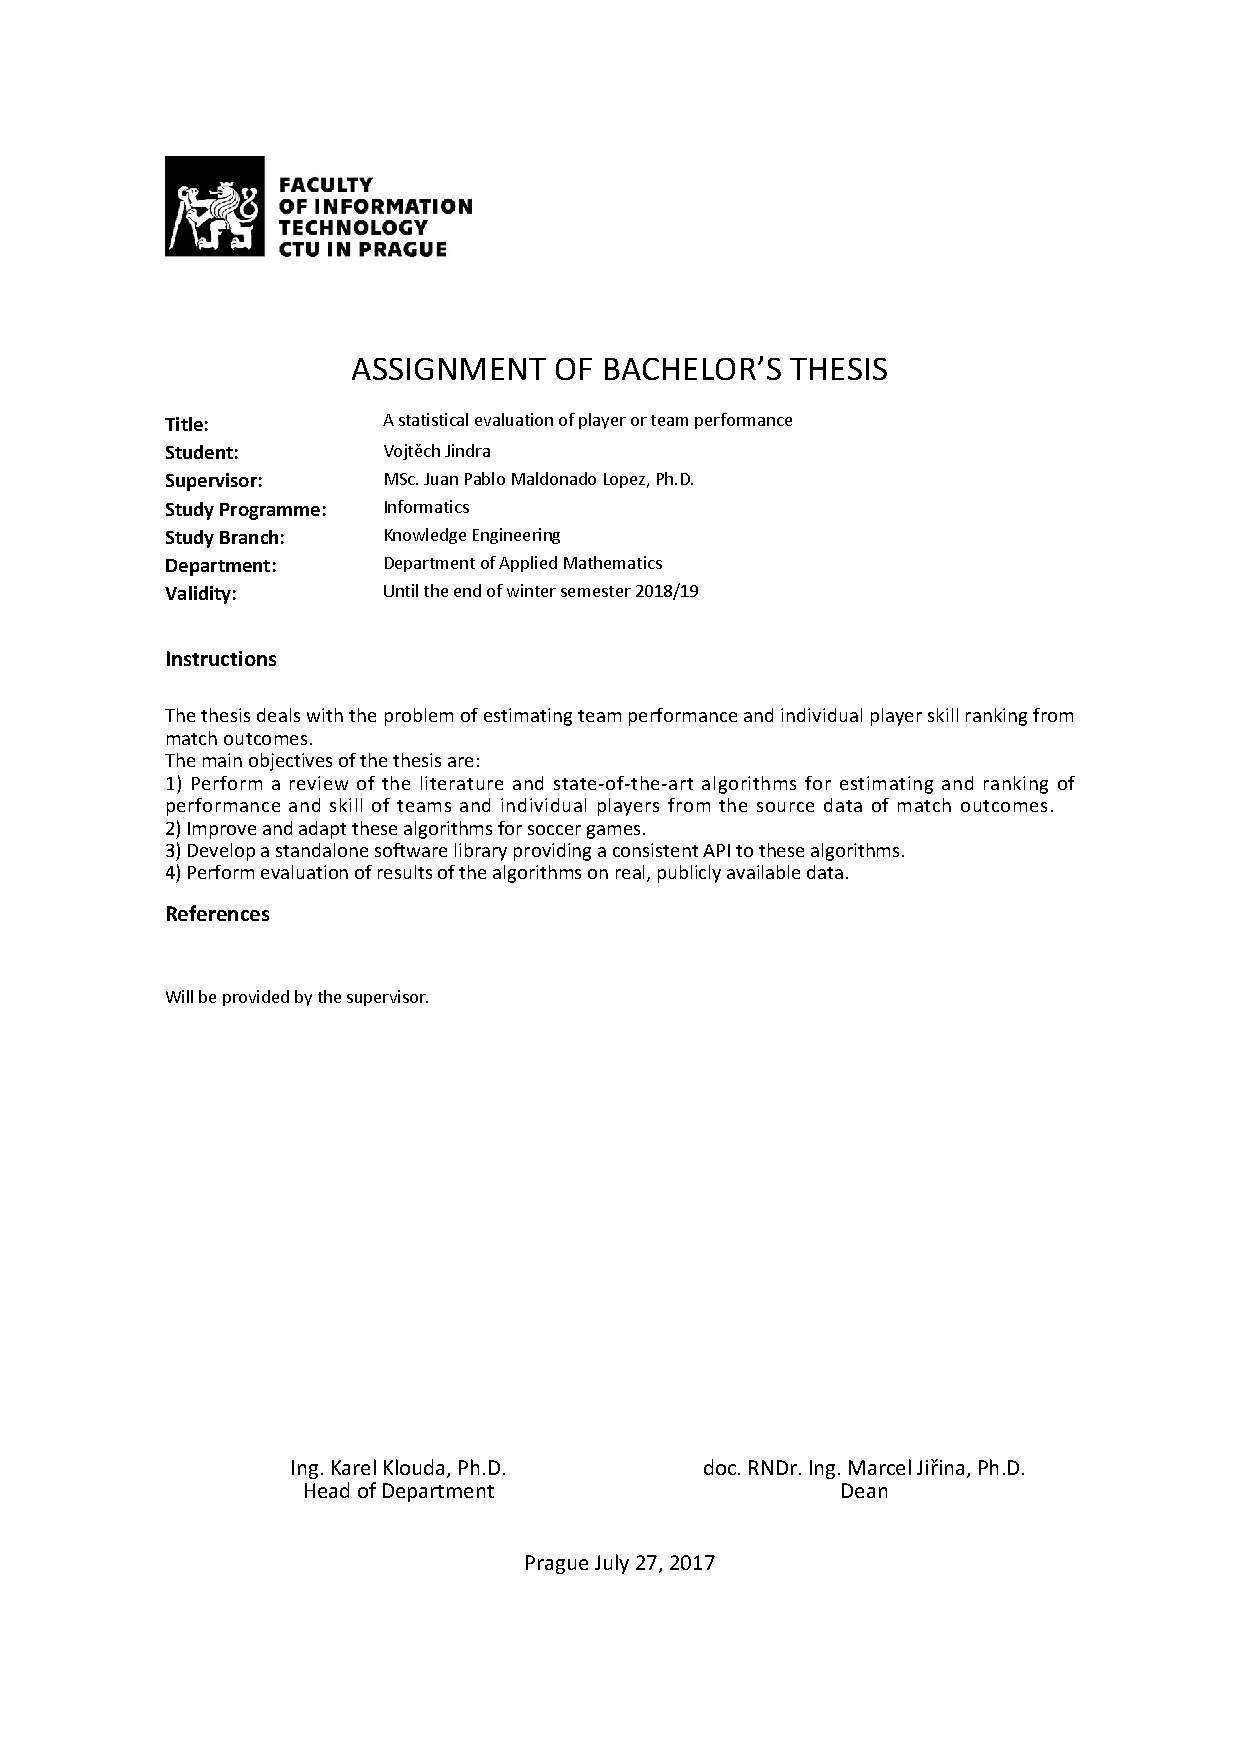
\includepdf[pages={1}]{assignment.pdf}
\newpage\null\thispagestyle{empty}\newpage

\maketitle

\chapter{Introduction}
\section{Problem statement}
Sports and games have been around the world forever. People used to decide, and still do, about their qualities based on all kinds of tournaments. 

Beating all other teams and winning tournaments seemed to be satisfying enough to decide what team is the best up until the year of 1959, when Arpad Elo came up with his statistical-based ranking algorithm for rating chess players \citep{Eloratingchessplayerspresent1978}. Except chess games, the algorithm has found its applications in different sports as well as in completely different fields.

Even though the Elo rating system has shown to be suitable for chess games, it had not necessarily found its way to other sports. People have come up with various ranking systems or variations of Elo in order to adapt to different sports. With the growth of massively multiplayer online computer gaming, much more sophisticated systems have been created to maximize the player's enjoyment gained from playing a game.

Rating systems introduce the possibility of building a ladder of players, reflecting their results and leading to increased competitiveness. Moreover, rating systems allow the game to match similarly strong players, leading to more balanced and therefore more enjoyable matches. Finally, the system's ability to predict future games can lead to interesting analyses. Overall, good rating systems improve the overall quality of a game leading to a better gaming experience, which obviously makes such game more desired.

Furthermore, rating systems are not limited to be used only in sports and gaming. As \citet{RainieUseOnlineRating2004} shows, plentiful of useful applications have been implemented, such as Google's famous PageRank algorithm \citep{PagePageRankcitationranking1998} used to rank quality of web pages, Amazon's products and sellers ratings \citep{ZhangMiningmillionsreviews2012} to detect the relevance of a product and reliability of a seller, or movie recommendation system used at Neflix \citep{FernandezRecommendationSystemNetflix2018}.

This thesis focuses on applications of several rating systems in soccer with the objective of improving their ability to predict future matches based on players' ratings. In order to achieve that, the results of numerous ranking algorithms are evaluated and then possible methods that lead to the improvement of the prediction ability are introduced. Finally, in \autoref{ch:realisation}, a description of the demo for ranking players and teams is provided, alongside with description of the API.

\section{Data analysis}
\label{sec:data_analysis}
Ranking algorithms are applied on soccer data taken from Kaggle's European Soccer Database, which provides the following \citep{EuropeanSoccerDatabase} data.
\begin{itemize}
\item Over 25 000 matches
\item Over 10 000 players
\item 11 European countries
\item Seasons from 2008 to 2016
\item Players' and teams' attributes
\item Team line up
\item Betting odds by bookkeepers
\item Detailed match events
\end{itemize}

Since not every match in the dataset is provided with all eleven players on each team, matches have to be checked for the suitability during preprocessing of the data, which leads to a final number of 21374 useful matches with following distribution of wins, loses and draws from the perspective of home team.

\begin{figure}[H]
\centering
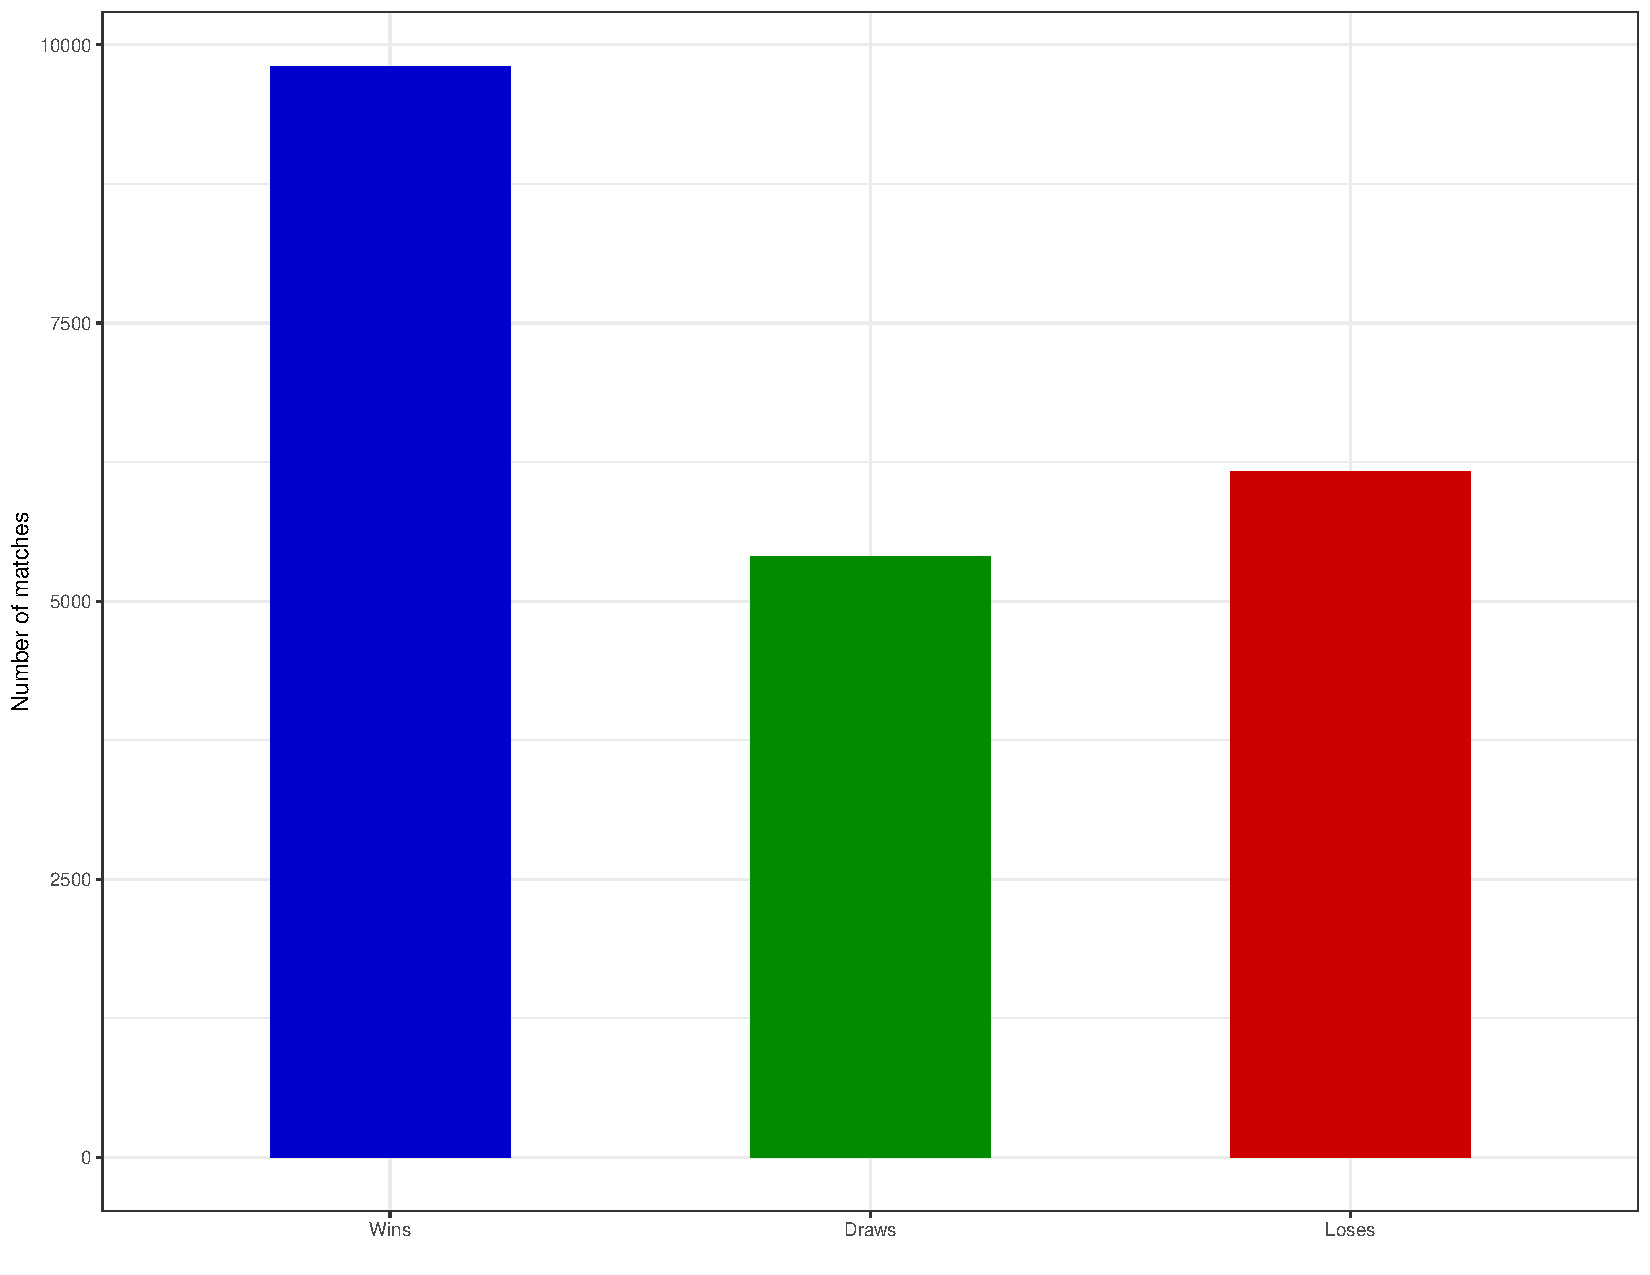
\includegraphics[width=.8\linewidth]{figs/match_distribution}
\caption{Distribution of outcomes}
\label{fig:match_distribution}
\end{figure}

It can be observed from the \autoref{fig:match_distribution} that teams playing on their home ground tend to win more matches. This is called the \textbf{home-team advantage} and is more thoroughly analyzed by \citet{BialkowskiWinHomeDraw}. To underpin the home-team advantage phenomena, distribution of scored goals throughout the matches follows.

\begin{figure}[H]
\begin{minipage}[b]{0.49\textwidth}
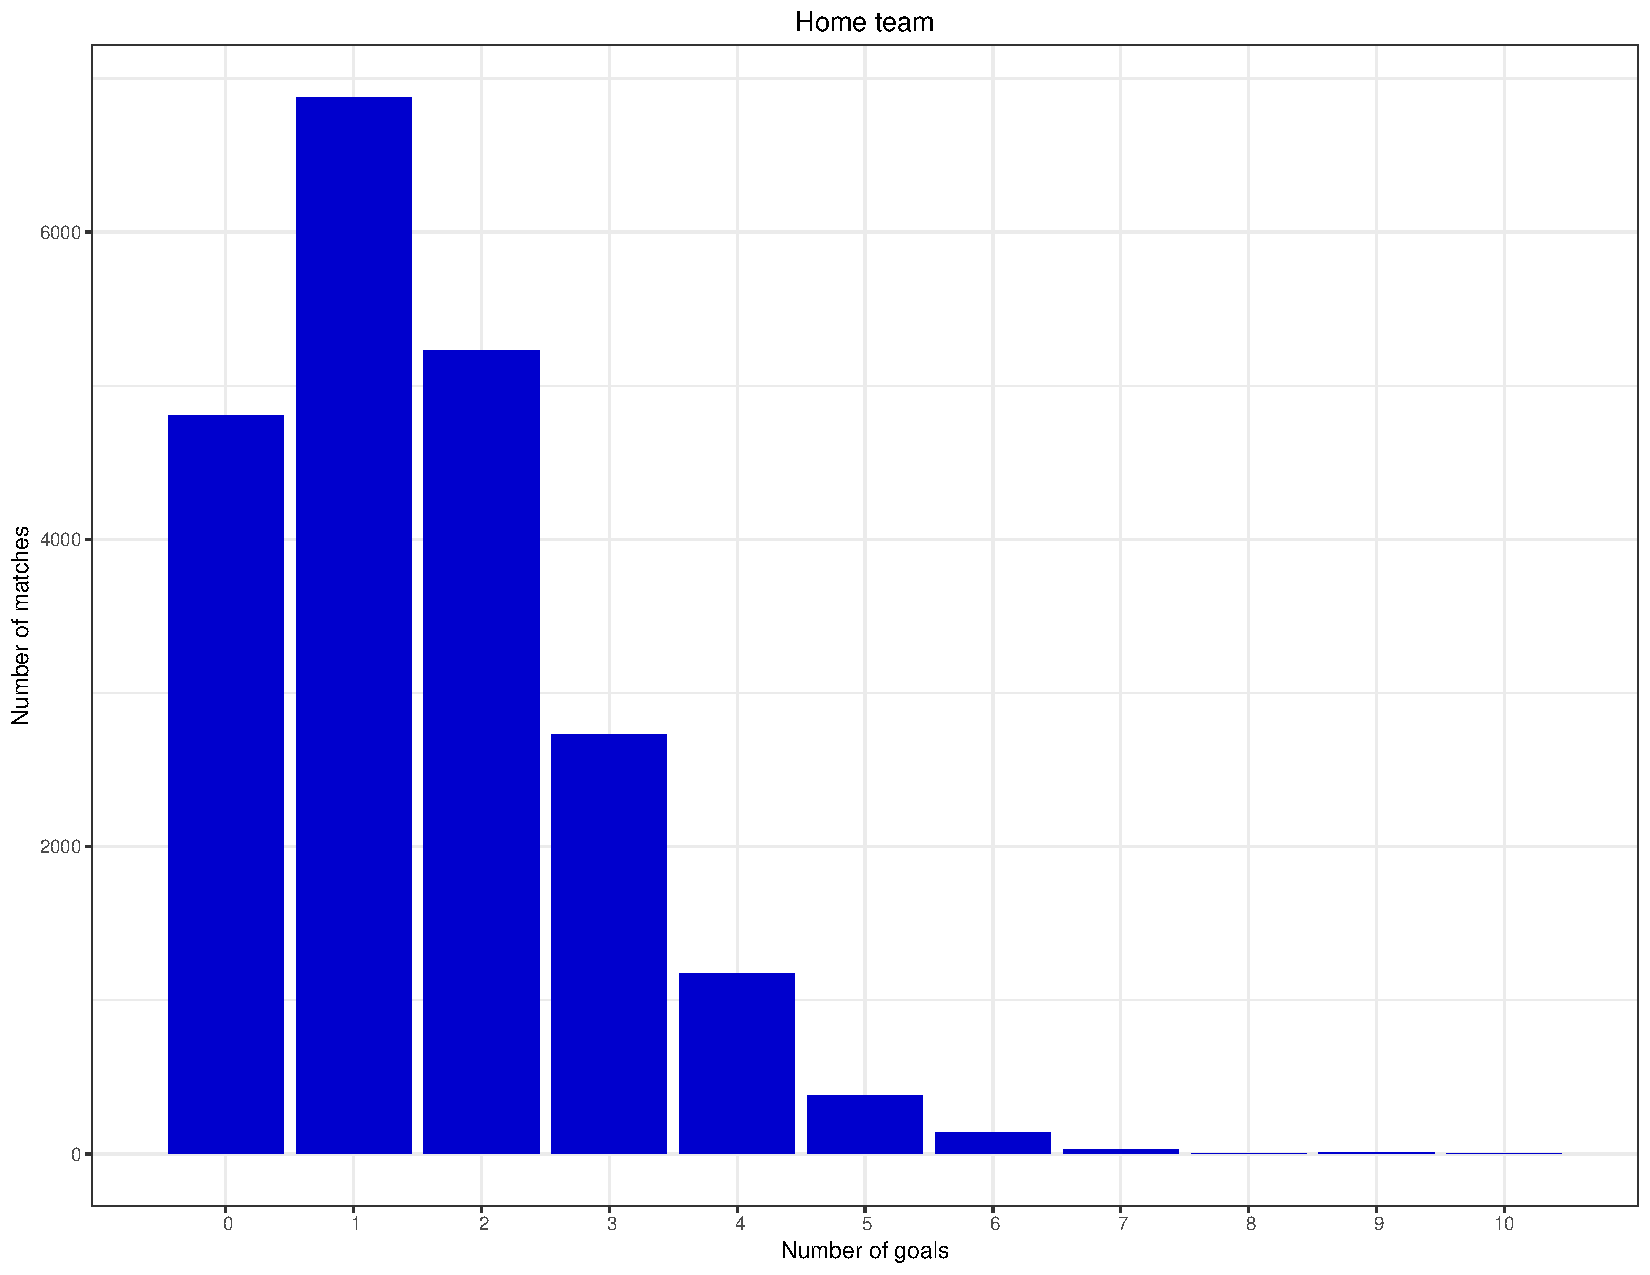
\includegraphics[width=\textwidth]{figs/goal_distribution_home}
\end{minipage}
\hfill
\begin{minipage}[b]{0.49\textwidth}
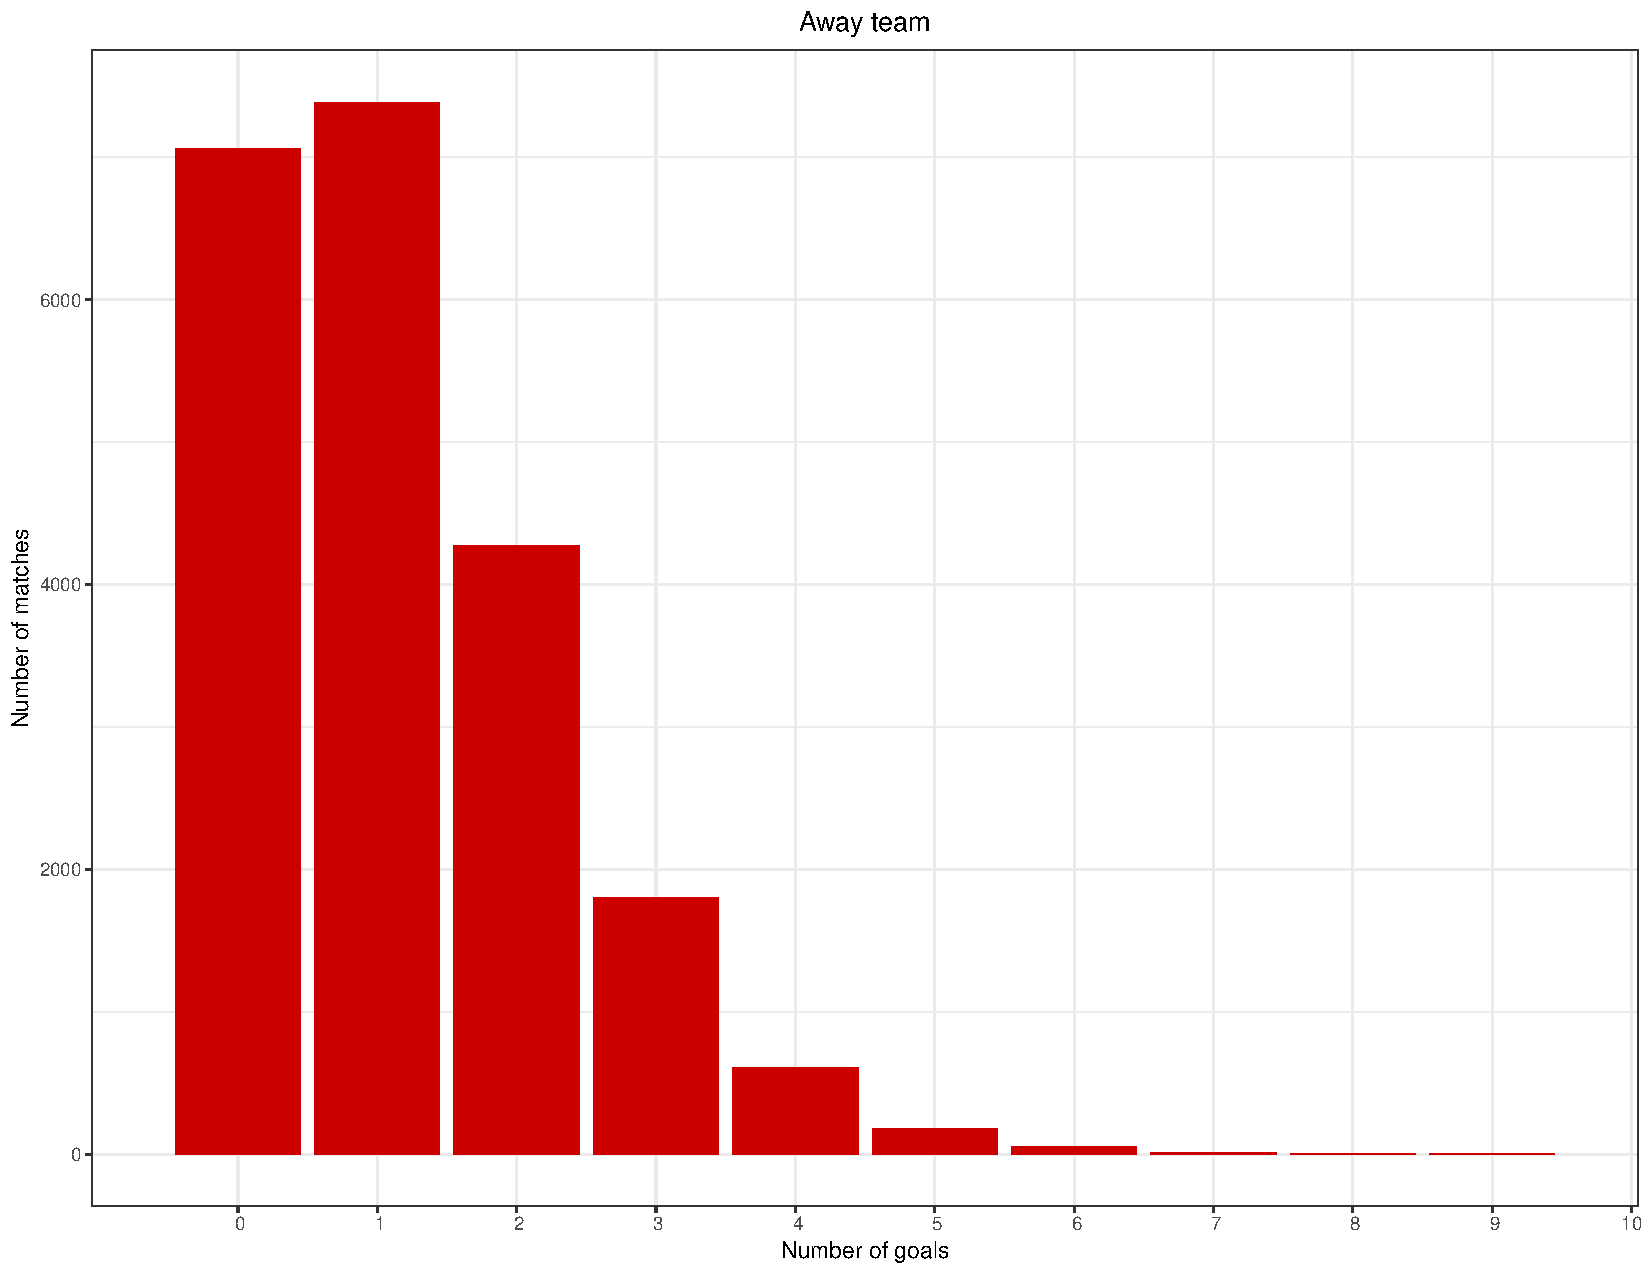
\includegraphics[width=\textwidth]{figs/goal_distribution_away}
\end{minipage}

\vspace{0.5cm}

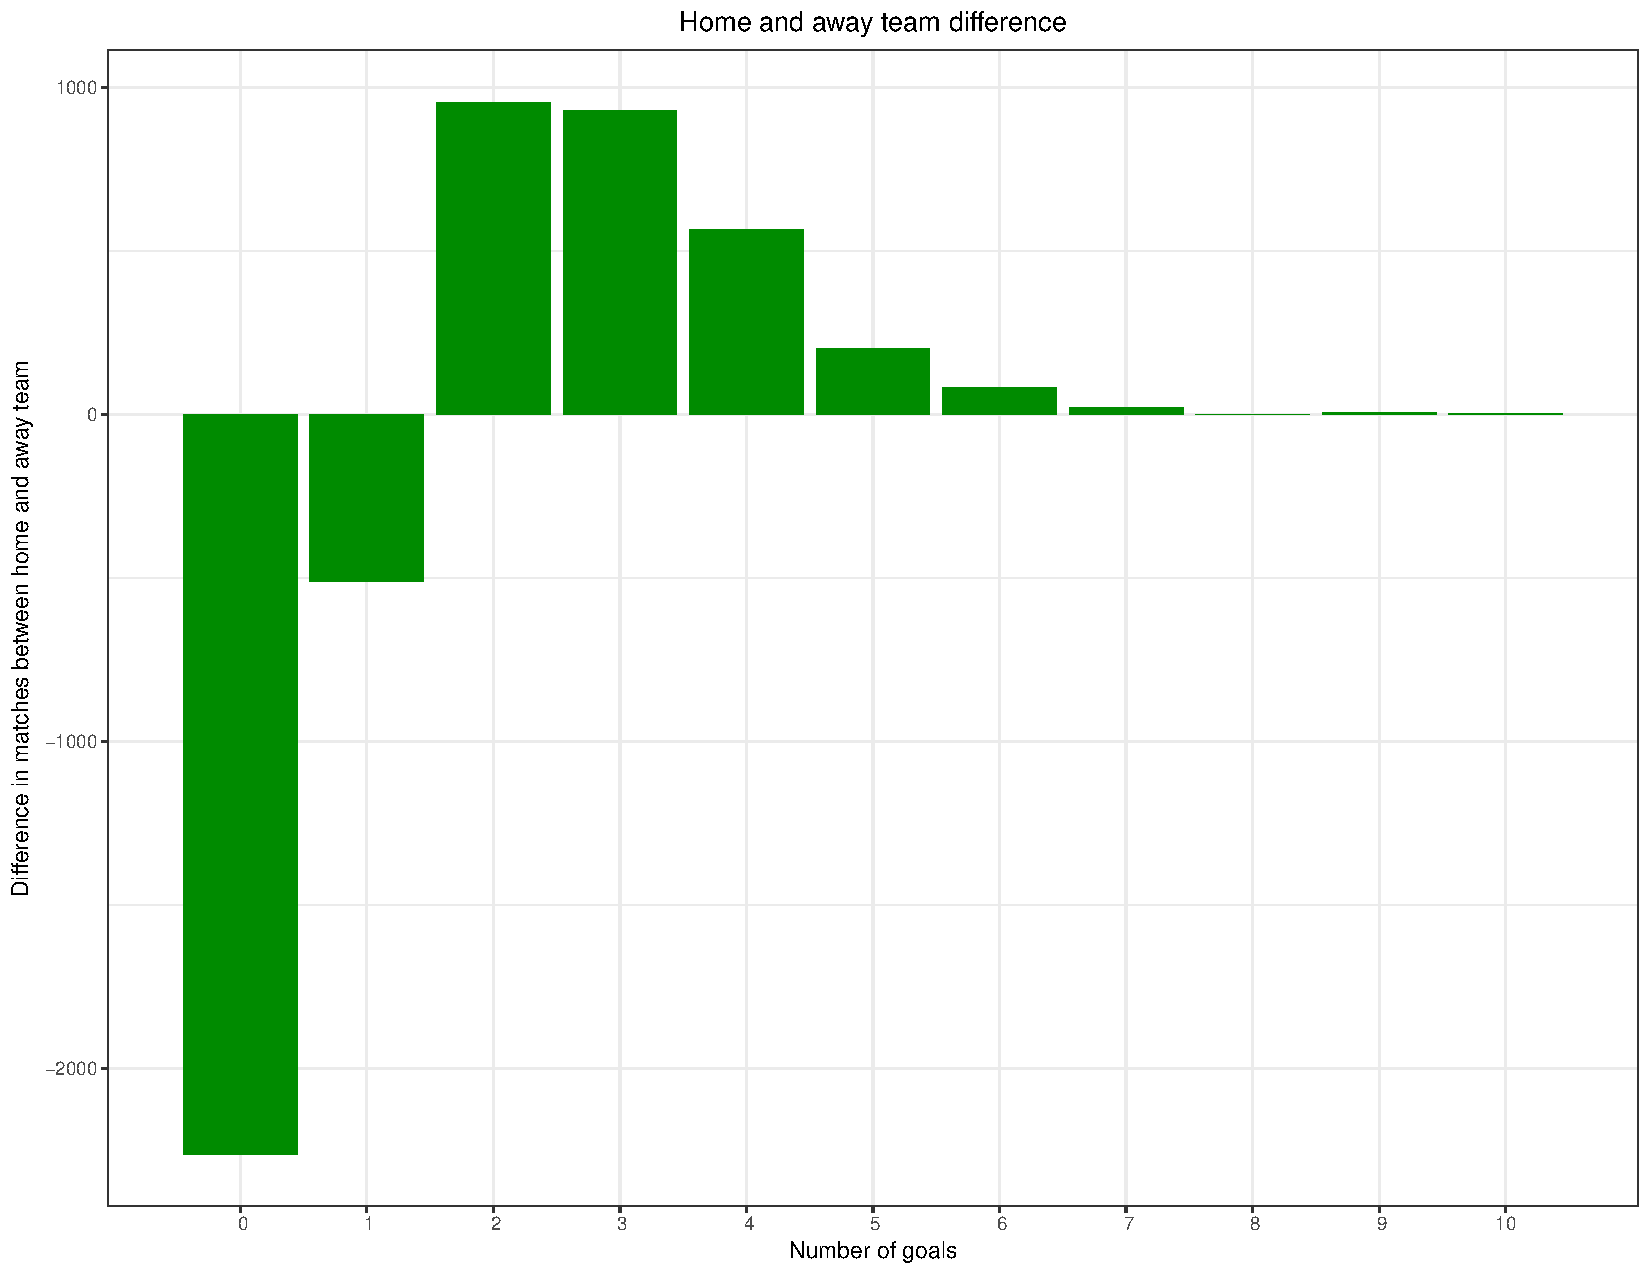
\includegraphics[width=.49\textwidth]{figs/goal_distribution}
\caption{Distribution of scored goals}
\end{figure}

Furthermore, while the away team scores only about $1.18$ goals on an average game, the home team manages to score $1.56$ goals.

Among the players' attributes provided by the dataset, there is the overall rating attribute, providing a rough estimation of player's overall skill based on his recent performance on a $[0, 100]$ scale. Such estimate can be normalized onto a more suitable interval to provide given algorithm with initial players' ratings, possibly leading to faster detection of their true skill.

\begin{figure}[H]
\centering
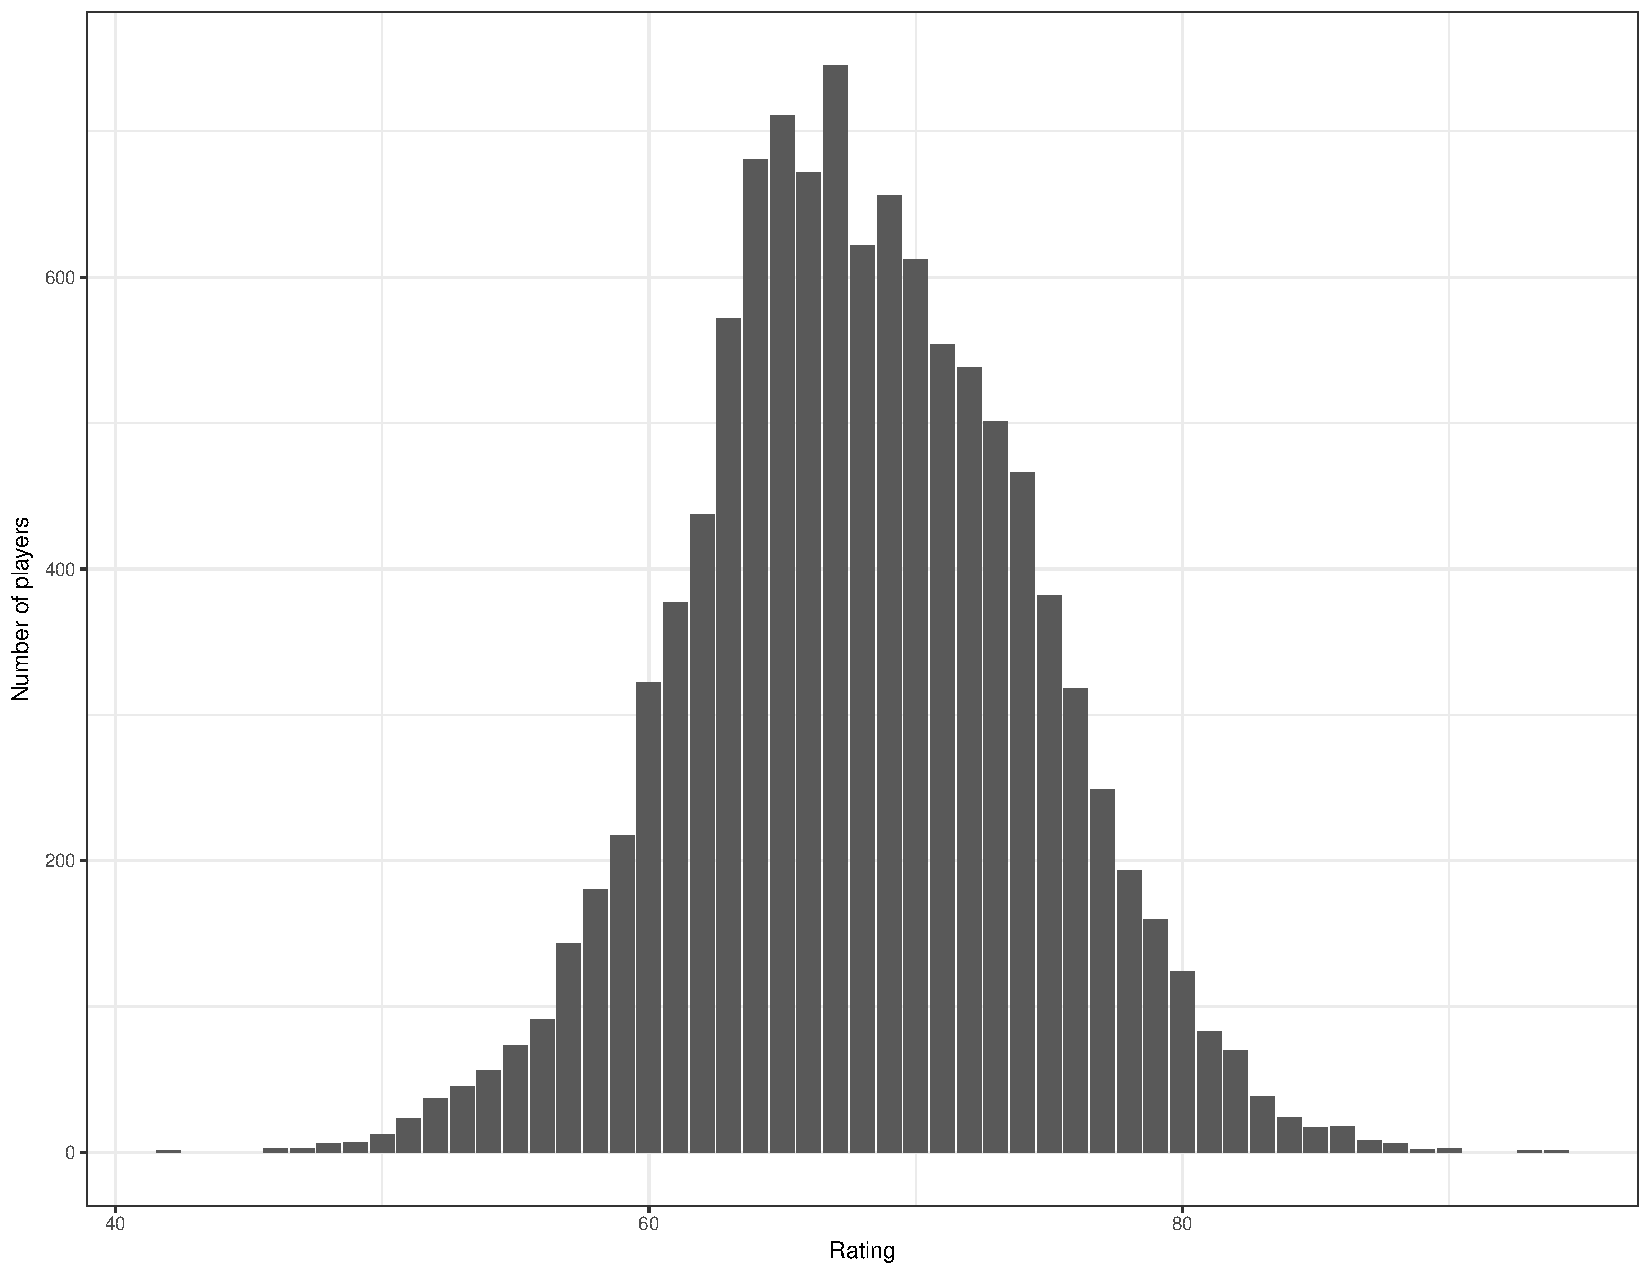
\includegraphics[width=.8\linewidth]{figs/overall_rating_distribution}
\caption{Distribution of overall rating attribute}
\end{figure}

An interesting follow-up statistic is the distribution of goals in given outcome for both home and away teams. \autoref{table:goals_per_outcome} shows such statistic recalculated to number of goals per game.

\begin{table}[H]
\caption{Table of goals per game with respect to outcome}
\label{table:goals_per_outcome}
\centering
\begin{tabular}{| r | c | c | c |}
\hline
& Win & Draw & Lose \\ \hline
Home team & 2.461 & 1.003 & 0.605 \\ \hline
Away team & 2.319 & 1.003 &  0.551 \\ \hline
\end{tabular}
\end{table}

Follows a graphical representation of the same statistic.

\begin{figure}[H]
\caption{Graphical representation of goals per game with respect to outcome}
\centering
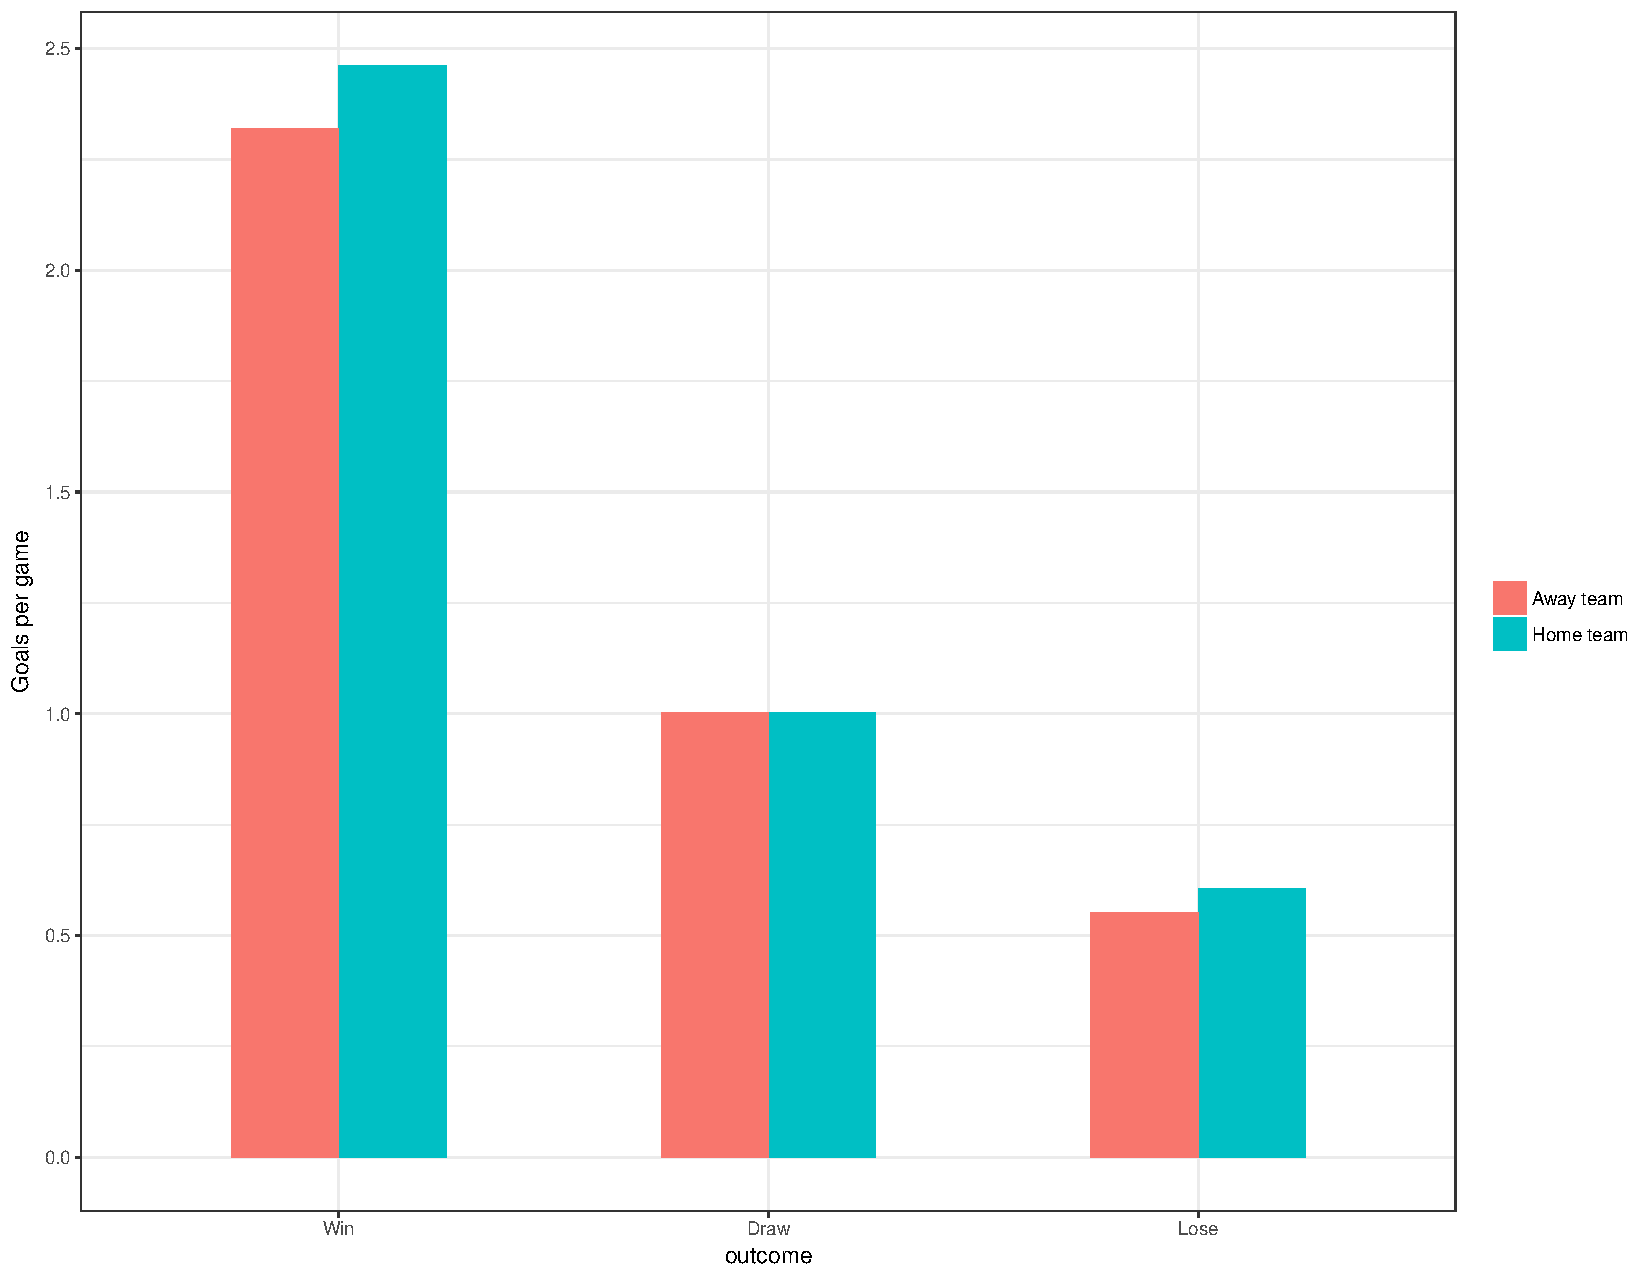
\includegraphics[width=0.8\textwidth]{figs/goals_per_game}
\end{figure}

\section{Measuring skill}
Before the description of specific rating systems, a brief introduction to skill measuring is relevant.

Skill is a relative measure that expresses how well does a player perform in given sport. When comparing two players, it is reasonable to say that the player with highest skill is more probable to defeat the other player. Therefore, skill can be perceived as a relative probability of winning, as introduced by \citet{BradleyRankAnalysisIncomplete1952}.

\begin{equation*}
P(i > j) = \frac{p_i}{p_i + p_j}.
\label{eq:bradley_terry}
\end{equation*}

The model expresses the preference of individual $i$ to individual $j$, with their skills represented as $p_i > 0$ and $p_j > 0$, respectively. A derivation of the Bradley-Terry model will be provided in \ref{sec:multilayer_perceptron}.

Measuring one's skill in games like chess is a lot more complicated than in other sports, where results can be interpreted using an absolute value. For instance, in 100 meter dash, the runner's skill is measured by the time he made. It does not matter who was he competing against, the time is an absolute measure to measure his skill by. However, in sports like chess, players compete against each other and the outcome strictly depends on the skill of player's opponent, which makes measurement methods such as number of victories totally unsuitable.

In order to measure skill of chess players, \textbf{rating} has been introduced. Rating is not measured in any units and therefore only provides information when compared to another player's rating. As capturing a player's skill by a single number may seem peculiar, note that perceiving rating as a random variable is much more appropriate. The number itself then represents the mean of the random variable's distribution, and therefore it is most probable that the player's true skill equals to his rating. The actual distribution of such random variable depends on the standard deviation, which can be variable according to the certainty of the system about the rating.

\examplespace
\begin{example}
Perceiving player's skill as a random variable of the standard normal distribution, skills of players A and B of ratings -0.4 and 0.7, respectively, could be visualized as follows.

\begin{figure}[H]
\centering
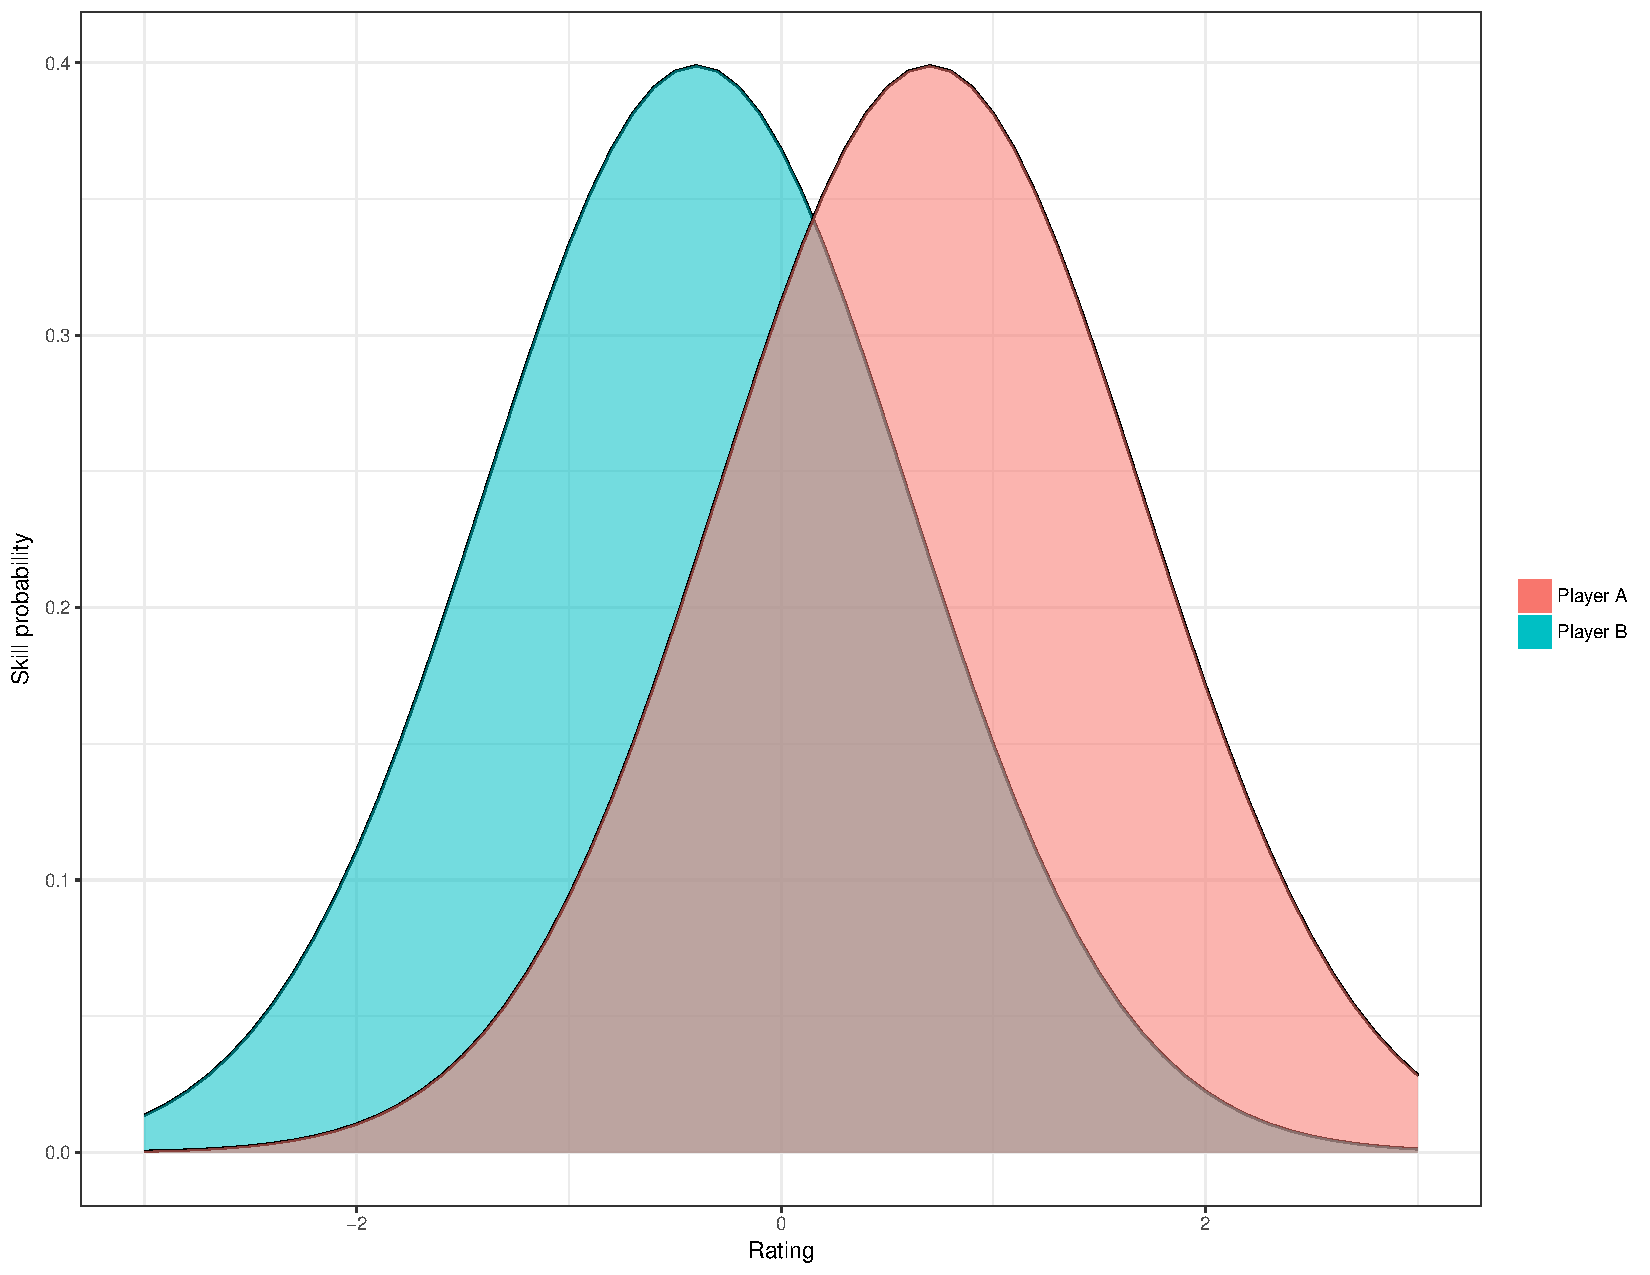
\includegraphics[width=.8\linewidth]{figs/players_skill_distribution}
\caption{Standard normal distribution of skills of players A and B}
\end{figure}

\noindent Hence the distribution of the outcome obtained by substracting distributions:
\begin{figure}[H]
\centering
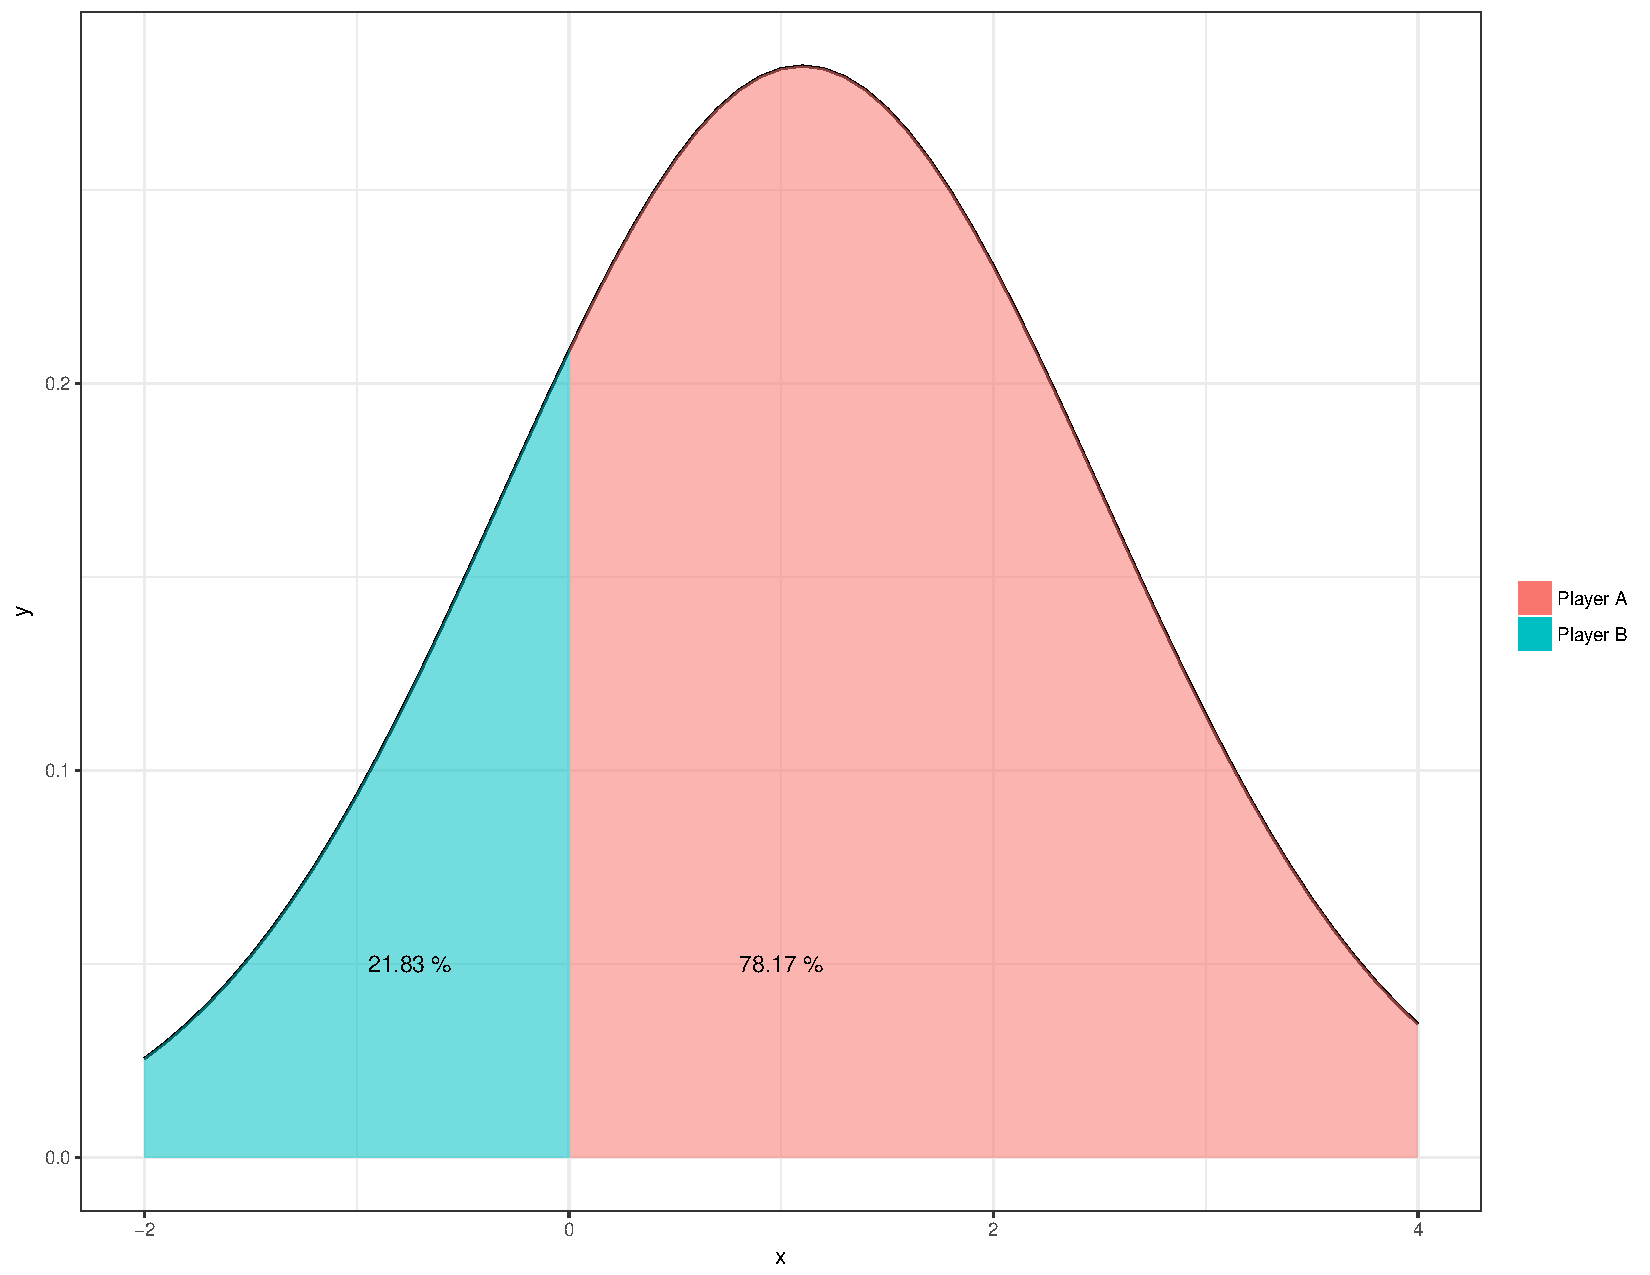
\includegraphics[width=.8\linewidth]{figs/outcome_distribution}
\caption{Distribution of outcome of a match}
\end{figure}

Therefore, the probability of player A defeating player B based on the certainty of their skills being -0.4 and 0.7, respectively, is 78.17\%.
\end{example}

\section{Outline of the thesis}
To complete the introductory chapter, we provide an overview of the chapters presented in the thesis. 

In \autoref{ch:online_ranking}, we will thoroughly describe the Elo algorithm followed by an extension for team ranking. Moreover, we will introduce several methods for improving the prediction ability of the Elo algorithm as well as techniques for adjusting the algorithm to used data.

In \autoref{ch:batch_ranking}, we will describe three algorithms that approach the problem of predicting outcomes of matches by processing previous matches. While the sections of Graph-based algorithms and Supervised Learning approach introduce state-of-the-art approaches for the task, the Maximum-likelihood method is our proposal for dealing with the problem statistics-wise.

In \autoref{ch:realisation}, we provide a description of the API of several ranking algorithms built for an easier access to the methods introduced throughout the thesis. The API is used in the demo web application to demonstrate its functionality. Moreover, a brief description of the scripts used to generate results as seen in the thesis is provided.

Finally, in \autoref{ch:conclusion}, we provide an overview of introduced algorithms followed by a conclusion derived from the work. Further, a table of results describing key features of said algorithms is presented alongside with their ability to predict outcomes of matches.
\chapter{Online ranking algorithms}
\label{ch:online_ranking}
\textbf{Online ranking algorithms} do not rely on obtaining information about all previous matches, they only need the last state of players' ratings to be able to update them. Therefore, they update players' ratings after every match that is played, not in a batch after some period.
 
The advantage of online ranking algorithms is that it is not required to process all matches when updating ratings, which can become computationally difficult for bigger datasets.

On the contrary, since all of the previous outcomes have to be captured by one state, it may become difficult to precisely capture all previous matches and some information may be lost.

\section{Elo for 2 players}
\label{ch:elo_for_two_players}
Elo is a ranking system used for 2-player games, originally in chess. It was introduced in 1959 by an amateur chess player Arpad Elo \citep{Eloratingchessplayerspresent1978}. It has been used in chess ever since, and because of its success and simplicity, people have started using Elo also for different sports.

The Elo ranking algorithm assumes that player's skill is normally distributed, with the mean of the distribution representing player's most probable skill. Although the original Elo system assumes a homogeneous normal distribution among all players, it was later observed that logistic distribution fits the chess data better \citep{ReganUnderstandingDistributionsChess2011} as well as it is computationally less complex. Therefore, the logistic distribution has been used for chess ratings.

\subsection{Expected score}
\label{sec:expected_score}
Elo's expected score equation is based on logistic function. It is used to calculate player's expected performance given both his and his opponent's ratings. The player's expected performance can also be viewed as his probability of defeating his opponent and it can be calculated as follows.

\begin{equation}
E_A = \frac{1}{1+10^\frac{R_B-R_A}{400}},
\label{eq:expected_score}
\end{equation}

\noindent with players $A$ and $B$ of ratings $R_A$ and $R_B$, respectively, expected score $E_A$ of player $A$ can be calculated.

As mentioned, the formula was originally based on logistic distribution, which assumes lesser chance of more extreme players winning/losing as shown in \autoref{fig:log_vs_normal}.

\begin{figure}[H]
\centering
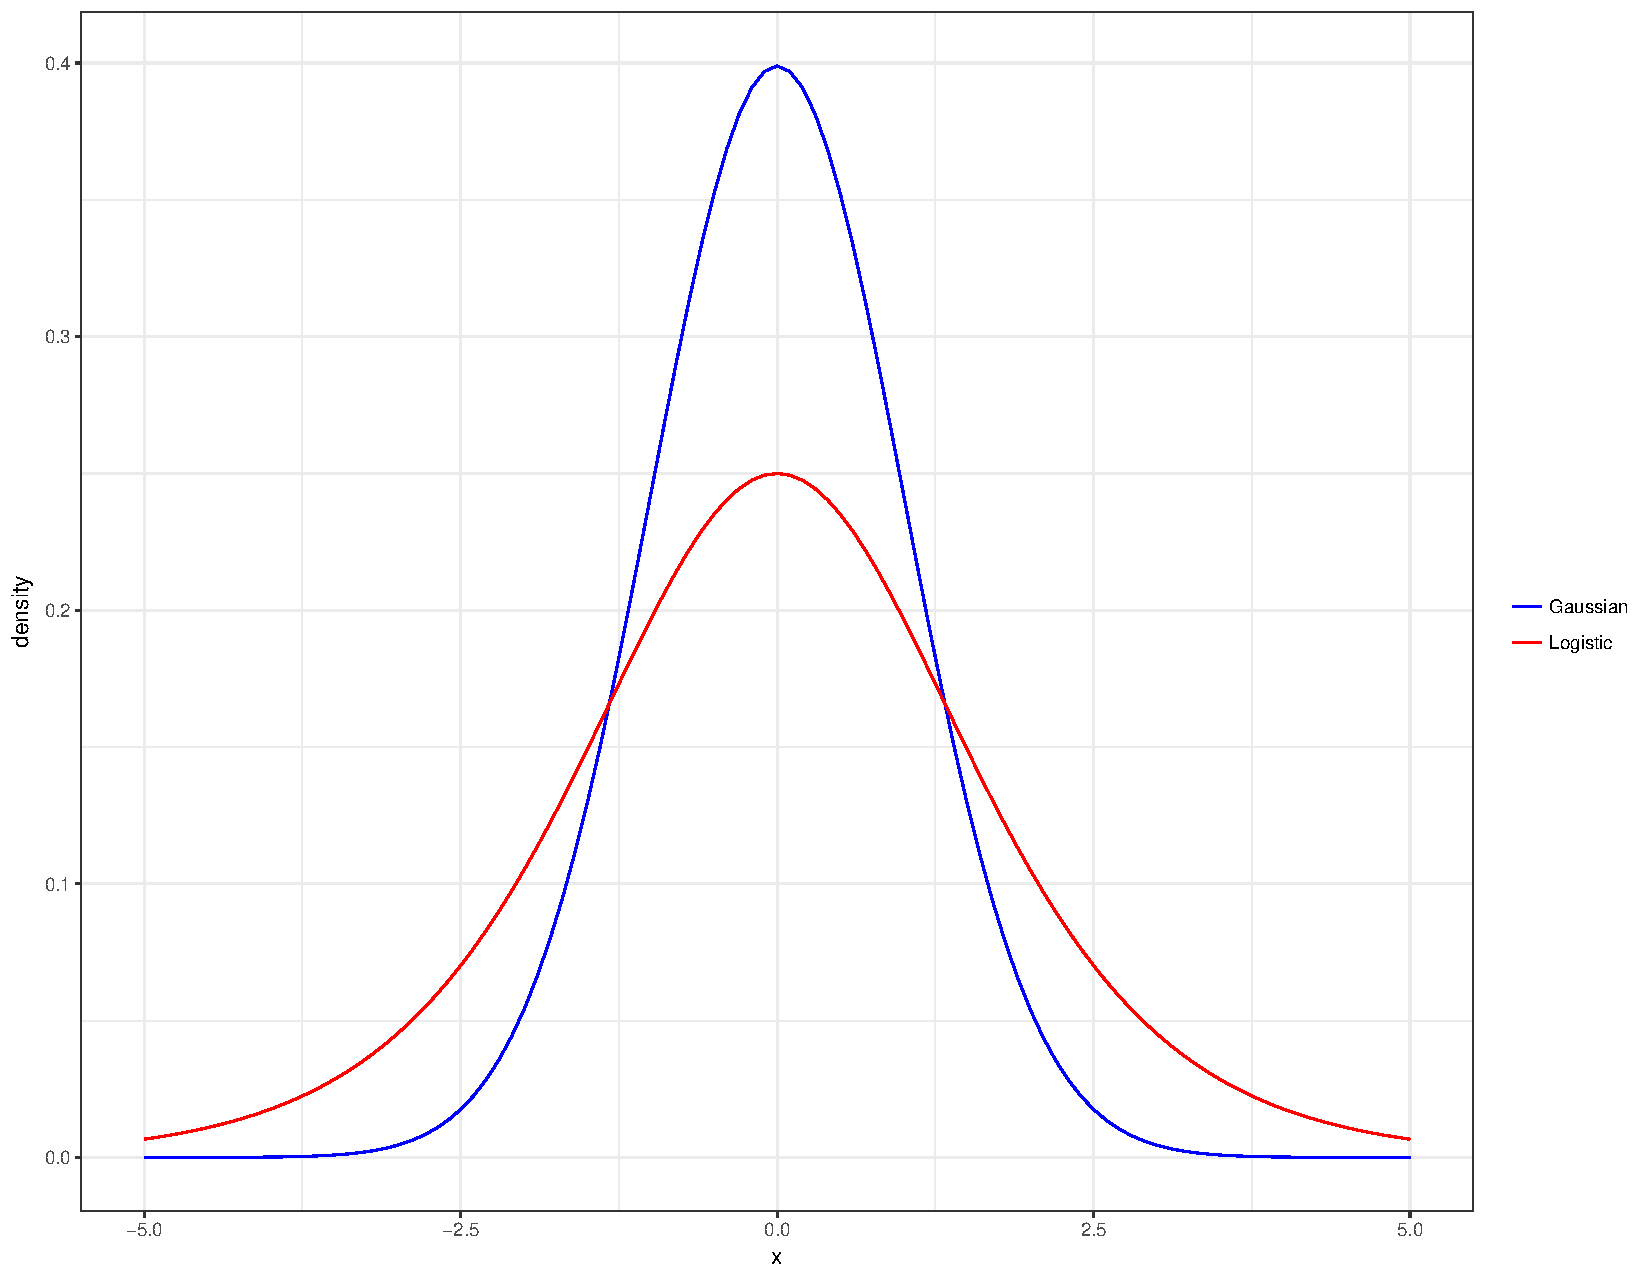
\includegraphics[width=0.8\textwidth]{figs/logistic_vs_gauss}
\caption{Difference between logistic and normal distribution}
\label{fig:log_vs_normal}
\end{figure}

The difference of 200 Elo points makes for a winning chance of \textasciitilde 76\% and is thought of as of a \textit{skill group}. The constants in the equation make the logistic function meet this rule as well as fit the actual chess players' data.

\begin{figure}[H]
\centering
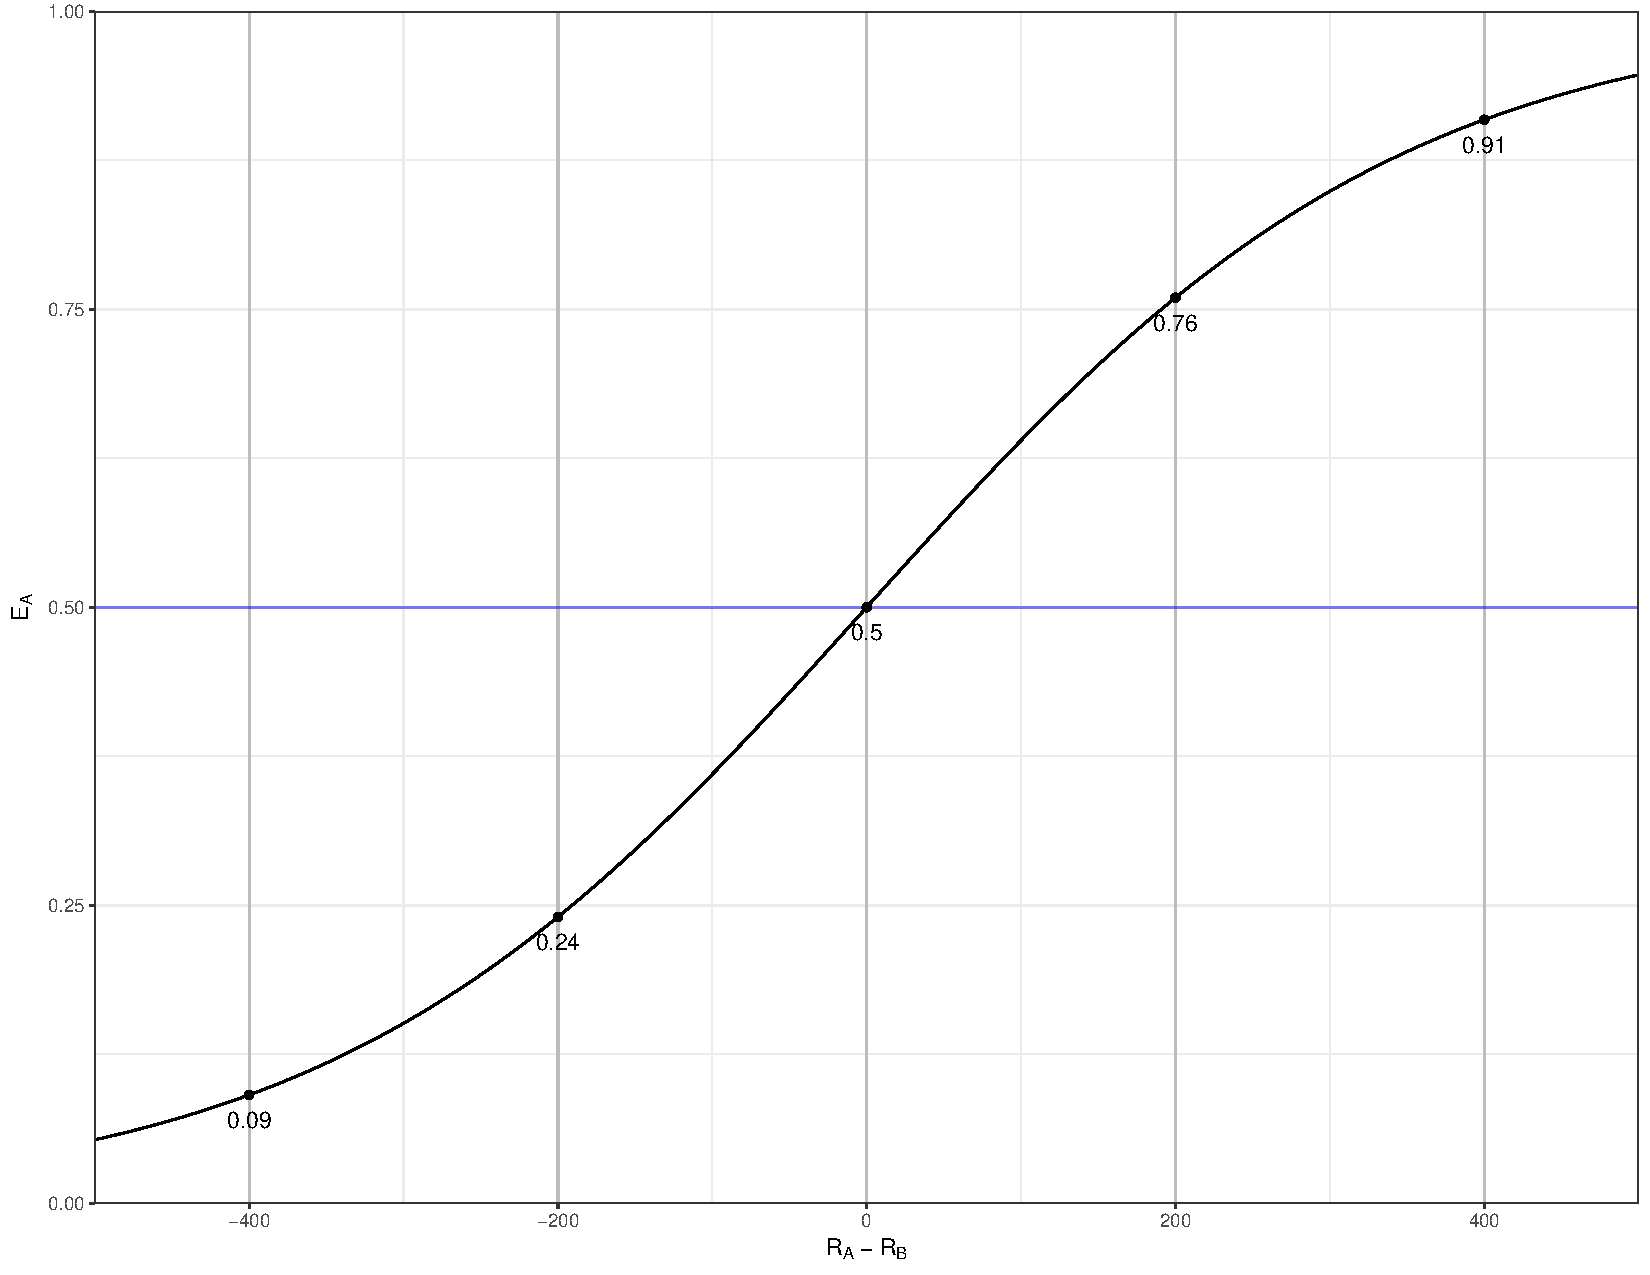
\includegraphics[width=0.8\textwidth]{figs/elo_logistic_function}
\label{Expected score equation}
\caption{Probability of winning based on rating difference}
\end{figure}

Since player's skill is thought of as a random variable, the logistic function can be perceived as the distribution of such random variable and therefore, a match of two players makes for a random variable of match's outcome and can be obtained by taking the difference of players' ratings.

Because $E_A$ and $E_B$ can be thought of as of probabilities of players $A$ and $B$ winning the game, it is intuitively a desired behavior that $E_A + E_B = 1$. The expected score formula, of course, meets this requirement.

Let $R_A$ and $R_B$ represent the rating of the players $A$ and $B$, respectively, then $E_A + E_B = 1$.

\begin{proof}
\begin{equation*}
\begin{aligned}
\frac{1}{1+10^{\frac{R_B-R_A}{400}}} + \frac{1}{1+10^{\frac{R_A-R_B}{400}}} &= 1\\[1em]
1+10^\frac{R_B-R_A}{400} + 1+10^\frac{R_A-R_B}{400} &= \left(1+10^\frac{R_B-R_A}{400}\right)\cdot\left(1+10^\frac{R_A-R_B}{400}\right)\\ [1em]
10^{\frac{R_B-R_A}{400}} \cdot 10^{\frac{R_A-R_B}{400}} &= 1\\[1em]
10^{\frac{R_B-R_A}{400} + \frac{R_A-R_B}{400}} &= 1\\[1em]
10^0 &= 1\\[1em]
1 &= 1
\end{aligned}
\end{equation*}
\end{proof}

Moreover, a little adjustment of the equation \eqref{eq:expected_score} reveals that Elo is a~derivation of the Bradley-Terry mode l\eqref{eq:bradley_terry}.

\begin{equation*}
\begin{aligned}
E_A &= \frac{1}{1 + 10^{\frac{R_B-R_A}{400}}} \\[1em]
&= \frac{1}{1 + 10^{\frac{R_B}{400}-\frac{R_A}{400}}} \\[1em]
&= \frac{1}{1 + \frac{10^{\frac{R_B}{400}}}{10^{\frac{R_A}{400}}}}\cdot \frac{10^{\frac{R_A}{400}}}{10^{\frac{R_A}{400}}} \\[1em]
&= \frac{10^{\frac{R_A}{400}}}{10^{\frac{R_A}{400}}+10^{\frac{R_B}{400}}} \\[1em]
&= \frac{p_A}{p_A + p_B}
\end{aligned}
\end{equation*}

Therefore, Elo is based on the Bradley-Terry model, with variables $p_A$ and $p_B$ representing scores of players $A$ and $B$, respectively. Therefore, in Elo, score of player $A$ is obtained as $10^\frac{R_A}{400}$, where $R_A$ holds his current rating.

\subsection{Updating ratings}
After the outcome of the game is known, players' ratings are updated accordingly. Intuitively, if a weak player beats a strong player, the weak player's rating should increase a lot, while the strong player's should decrease a lot. Similarly, if a strong player defeats a weak player, the weaker player should not be punished that much. In other words, results that are expected by the system should not lead to big changes in players' ratings, while unexpected results should.

In the Elo, following equation is used to update player's rating

\begin{equation}
R_A' = R_A + K(S_A - E_A),
\label{eq:update_equation}
\end{equation}

\noindent where $R_A$ is player's rating before the update, $E_A$ is player's expected score calculated from expected score formula \eqref{eq:expected_score} and $S_A$ is player's actual score, which can hold 3 different values:

\begin{itemize}
\item $1$ if player A won, 
\item $0$ if he lost,
\item $0.5$ if the game ended in a draw.
\end{itemize}

Finally, the $K$ is called $K$ factor and represents the maximum value a player can either lose or gain. The $K$ factor can vary depending on player's rating as described in \eqref{sec:k_factor}.

The equation \eqref{eq:update_equation} fits the requirements for an update formula as more unexpected results lead to more extreme changes while predictable results update the ratings by lower values.

In \autoref{fig:k_factor}, the change in player's rating based on difference of both players' ratings using $K$ factor of 32 is indicated.

\begin{figure}[H]
\centering
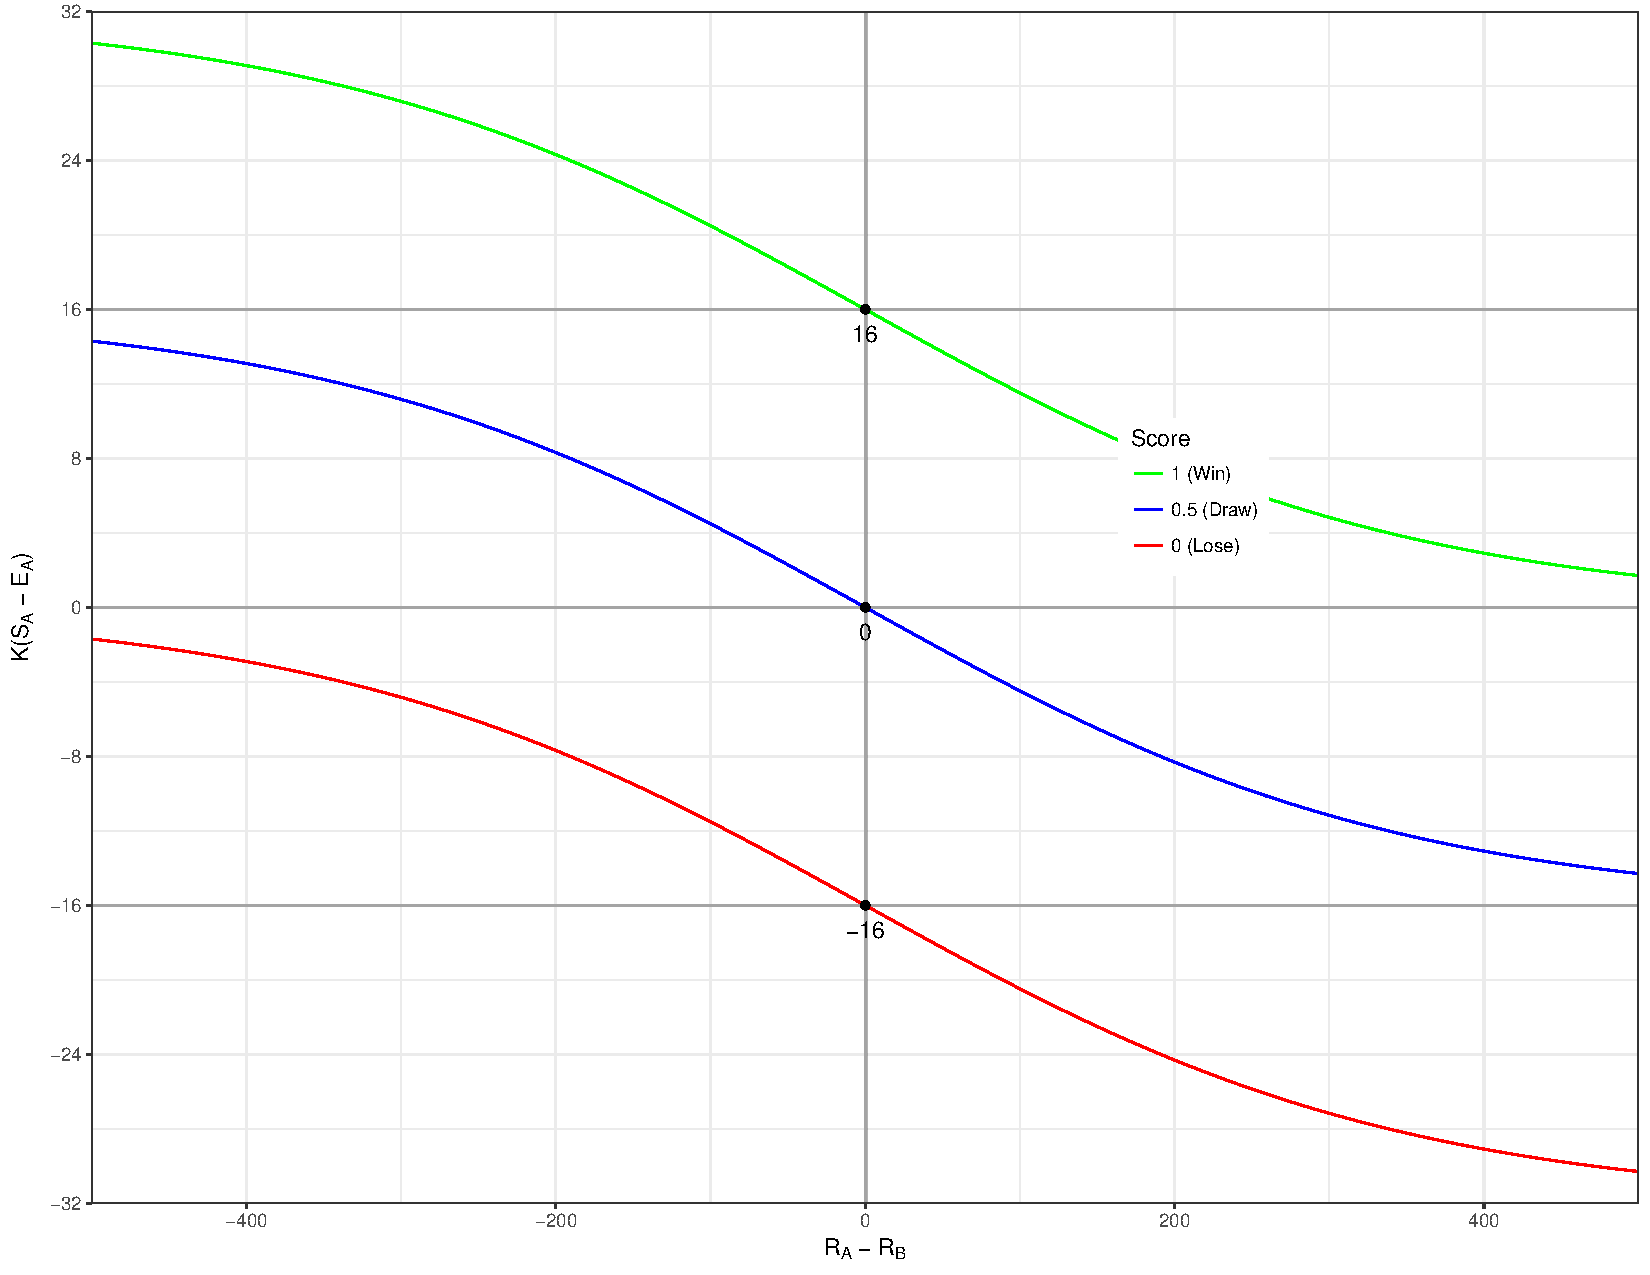
\includegraphics[width=0.8\textwidth]{figs/elo_k_factor}
\caption{Change in rating for K factor of 32}
\label{fig:k_factor}
\end{figure}

\subsection{K factor}
\label{sec:k_factor}
As the $K$ factor defines the maximum possible update of a player's rating after one game, having such parameter fixed leads to the lack of ability to recognize player's true skill in shorter time and dynamically respond to that. To provide an example, player's increased number of victories likely points to player's higher true skill, since he tends to defeat players with ratings similar to his. The system should be able to react to such situations by increasing the player's rating by higher values until he eventually reaches his true skill and stabilizes.

The USCF and FIDE solve this by dividing players into three categories based on their rating and setting a different value of $K$ factor for every category. That makes it easier for new players to achieve rating according to their actual skill and once their rating reaches a pre-set value, they get artificially settled by setting their $K$ factor to a lower value. Note that FIDE sets $K$ factor to 10 after a player reaches rating of 2400 and then the player is considered settled, therefore his $K$ factor stays at 10 even if the player manages to reduce his rating back under 2400.

\examplespace
\begin{example}
For an example of the Elo rating system, let's have a match of two imaginary players Alice and Bob with ratings 1170 and 1290, respectively. The probability of Alice defeating Bob $E_A$ will be calculated as follows.

\begin{align*}
E_A &= \frac{1}{1+10^{\frac{R_B-R_A}{400}}} \\
&= \frac{1}{1+10^{\frac{1290-1170}{400}}} \\ 
&= \frac{1}{1+10^{\frac{120}{400}}} \\[0.5em]
&\doteq 0.334
\end{align*}

Therefore, Alice's chances of beating Bob are around 33.4\%. Complementarily, Bob's chances are about 66.6\%. Let's say Alice beats her odds and defeats Bob. Assuming $K$ factor of 32, her rating will be update as follows. 

\begin{align*}
R_A' &= R_A + K(S_A - E_A) \\
&= 1170 + 32(1 - 0.334) \\
&\doteq 1191.3
\end{align*}

In the same spirit, Bob's rating will decrease as follows.

\begin{align*}
R_A' &= R_A + K(S_A - E_A) \\
&= 1290 + 32(0 - 0.666) \\
&\doteq 1268.7
\end{align*}

If they were to play the same match again with updated ratings, the system would expect Alice to defeat Bob with a \textasciitilde 39\% chance.
\end{example}

\section{Extensions to the Elo algorithm}
\label{section:elo_for_teams}
In this chapter we provide a heuristic algorithm to derive an extension of the Elo ranking algorithm for teams with multiple players. This consists of computing individual player Elo scores and aggregating them to produce an Elo score for the team. Winning likelihoods are then computed.

\subsection{Altering the classification rule by number of draws}
As the Bradley-Terry model is used for calculating expected score in the Elo ranking system, only probabilities of winning or losing can be obtained. However, in sports, it is often desired for draws to be considered. As \citet{RaoTiesPairedComparisonExperiments1967} suggested, the Bradley-Terry model can be extended to account for ties by introducing $\theta \geq 1$ parameter. Then, the Rao-Kupper model captures the preference of $i$-th player over $j$-th player and vice versa in dependence on their skills $\pi_i$, $\pi_j$, respectively, as

\begin{align*}
P(i > j) &= \frac{\pi_i}{\pi_i + \theta\pi_j},\\
P(j > i) &= \frac{\pi_j}{\pi_j + \theta\pi_i}
\end{align*}

\noindent and the probability of a game between $i$-th and $j$-th player resulting in a tie can be expressed as

\begin{align*}
P(i = j) = \frac{(\theta^2 - 1)\pi_i\pi_j}{(\pi_i+\theta\pi_j)(\pi_j+\theta\pi_i)}.
\end{align*}

The $\theta$ parameter is chosen accordingly to the frequency of ties in given sport. While in soccer draw is a common outcome of a match and therefore the $\theta$ is desired to be high, for instance in Olympic swimming, swimmers are considered to draw if their times are tied to a hundredth of a second, making draws much less often. Hence, for swimming, the $\theta$ parameter should be smaller, making prediction of a draw less probable.

To obtain the $\theta$ parameter for the data used throughout this thesis, minimization of function $f(\theta)$ as shown in \eqref{eq:rao_kupper_minimization} has been performed.

\begin{align}
\label{eq:rao_kupper_minimization}
f(\theta) = \frac{1}{|M|}\nsum_{i \in M}{
\begin{bmatrix}
o_{i_w} & o_{i_\ell} & o_{i_d}
\end{bmatrix}
\times
\begin{bmatrix}
p_{i_w}\cdot\log{p_{i_w}} \\
p_{i_\ell}\cdot\log{p_{i_\ell}} \\
p_{i_d}\cdot\log{p_{i_d}}
\end{bmatrix}
},
\end{align}

where $i \in M$ denotes $i$-th match from the set of all matches $M$, $o_{i_w}$, $o_{i_\ell}$, $o_{i_d}$ its outcome in the sense that $o_{i_w} = 1, o_{i_\ell} = o_{i_d} = 0$ if the team won and correspondingly for loses and draws, and $p_{i_w}$, $p_{i_\ell}$, $p_{i_d}$ probabilities of winning, losing and drawing, respectively, predicted by the Rao-Kupper model.

By minimizing $f(\theta)$, a result of $\theta \doteq 1.326$ has been obtained. However, we believe that the draws in used dataset are not sufficiently significant and the obtained result does not reflect the reality, making the Rao-Kupper model unusable for the dataset. To support the statement, probability of a draw of two players $i$ and $j$ of equal ratings $R_i = R_j = 1200$ is calculated using $\theta = 1.326$:

\begin{align*}
P(i = j) &= \frac{\left(1.326^2 - 1\right)10^{1200/400}10^{1200/400}}{\left(10^{1200/400}+1.326\cdot 10^{1200/400}\right) \left( 10^{1200/400}+1.326\cdot 10^{1200/400}\right) } \\[1em]
&\doteq 0.14.
\end{align*}

While the probability of a draw is at its peak for a match of players of equal ratings, the probability has been calculated to 14\%. For players of different ratings, the probability will only get lower. However, draws make up for a total of \textasciitilde 23\% of all matches in the dataset, pointing to a conclusion that Rao-Kupper is not usable for our dataset.

\subsection{Parameter optimization for prediction}
Since the Elo algorithm was adjusted to fit the chess data, the expected score equation \eqref{eq:expected_score} uses two constants that we try to adjust accordingly to soccer data. In order to do that, we maximize the prediction ability of expected score equation using derivative-free methods.

\subsubsection{Simulated annealing}
\label{sec:simulated_annealing}
Simulated annealing is a probabilistic technique for finding the global optimum of a function introduced by \citet{KirkpatrickOptimizationSimulatedAnnealing1983}. The algorithm starts with an initial temperature and while searching the space, it slowly cools down. With lower temperature comes lower probability of getting stuck in a local optimum. Therefore, the algorithm tends to neglect local optima. When the algorithm cools down, making it unable to escape local optima, it stops.

More thorough explanation of the simulated annealing algorithm is provided in \autoref{ch:simulated_annealing}.

After determining players' ratings, simulated annealing algorithm is used to alter the expected score equation \eqref{eq:expected_score} to maximize number of correctly predicted matches. Therefore, $x$ and $y$ in formula \eqref{eq:expected_score_altered} are adjusted in order to maximize algorithm's prediction ability.

\begin{equation}
\label{eq:expected_score_altered}
E'_A = \frac{1}{1+x^\frac{R_B-R_A}{y}}.
\end{equation}

Another approach is to minimize the formula's log-likelihood loss function \citep{BujaLossFunctionsBinary2005} using simulated annealing. Although, log-likelihood loss function and number of correctly predicted matches tend to be correlated, and therefore both approaches lead to similar results.

\subsubsection{Cross-entropy method}
Cross-entropy method is a Monte Carlo approach to global optimization introduced by  \citet{RubinsteinCrossEntropyMethodCombinatorial1999}. In order to find the global optimum, a random data sample is generated according to a parameter, from which only the most elite percentage is chosen and the parameter to generate the data sample with is updated according to the elite. This process is repeated multiple times to obtain the global optimum.

Again, more detailed information on cross-entropy method can be read at \autoref{ch:cross_entropy_method}.

In the case of optimizing Elo's parameters, 100 random samples from a two dimensional normal distribution with the Elo's equation's constants $x$ and $y$ from \eqref{eq:expected_score_altered} is generated and the average of the most elite 20\% of such is used to update the parameters. This process is repeated 100 times.

To optimize Elo's parameters using cross-entropy method, the cross-entropy error function \citep{deBoerTutorialCrossEntropyMethod2005} of correctly predicted matches is used as the fitness function. The cross-entropy error function in general case looks as follows.

\begin{equation*}
H(p, q) = -\sum_i{p_i\log{q_i}}.
\end{equation*}

And therefore, for Elo's parameter optimization:

\begin{equation*}
H(w, p) = -\sum_i{(w_i\cdot\log{p_i} + (1-w_i)\cdot\log{(1-p_i)})},
\end{equation*}

\noindent where $w_i$ equals to 1 if the home team won the match, 0 otherwise, and $p_i$ is the probability of home team winning the game predicted by the Elo model.

Since both of those algorithms are used to find the global maximum of the Elo's equation, they both had similar results. Again, since there is a fair amount of randomness included, there is no point in saying whether one of them was slightly better.

\subsection{Using normal distribution}
Although the Elo rating system follows the logistic distribution for calculating expected score of a player, as mentioned in \ref{sec:expected_score}, the original formula proposed by Arpad Elo used a normal distribution. The reason it was disregarded in favor of logistic distribution was that the latter captured the chess data more accurately.

Because we use soccer data, it is reasonable to use the normal distribution $\mathcal{N}(\mu, (2000/7)^2)$ proposed by Arpad Elo. The distribution assumes that players' ratings are homogeneously distributed and uses a constant deviation $\sigma=\frac{2000}{7}$. The mean $\mu$ is equal to given player's rating.

\subsection{Treating teams as individuals}
An intuitive way to extend the Elo algorithm to be able to calculate team ratings is to treat every team as an individual. This approach leads to having team rating based purely on match outcomes with no respect to the team's players' individual skills. Therefore, with unstable team lineups, predicting future games turns out to be challenging. 

Although, to provide an intuitive comparison to the approach presented in \ref{sec:elo_team_ranking}, real data has been evaluated using this approach as well.

\subsection{Adaption for team ranking}
\label{sec:elo_team_ranking}
To extend Elo to be able to rank teams, teams are perceived as individual players. However, team ratings are determined from individual players' ratings and after the team's rating is updated, the update is propagated back to players' ratings. The propagation has to ensure consistency of ratings, i.e. the rule applied to calculate team's rating from players' ratings has to be applicable and equivalent to the team's updated rating after the update.

\subsubsection{Obtaining team's rating}
The goal of obtaining team's rating is to obtain such rating that captures the team's skill (i.e. its players' joined skills) as accurately as possible. It may seem useful to introduce new attributes of the obtained rating, for example deviation of players' ratings, but it is essential to use the rest of the Elo formulas without further complicated alterations.

Therefore, we obtain team's rating by calculating arithmetic mean of all players' ratings that belong to the team. This lets the team's rating remain on the same scale as players' ratings and therefore be suitable for other Elo equations without further adaptations. Also, every player's rating affects the team's rating equally. A downside of such approach is the difficulty of comparing quantitatively unbalanced teams. Although, quantitatively unbalanced soccer matches are rare and therefore we believe that formula \eqref{eq:obtaining_teams_rating} is suitable for calculating team's rating.

\begin{equation}
\label{eq:obtaining_teams_rating}
R_{T_i} = \frac{1}{|T_i|}\sum_{R_j \in T_i}{R_j},
\end{equation}

\noindent where $T_i$ is a set of all ratings of all players in $i$-th team and $|T_i|$ is size of such set (i.e. number of players in the team).

\subsubsection{Applying Elo's equations}
The obtained teams' ratings can be treated as ratings of individuals and therefore expected score equation \eqref{eq:expected_score} and update equation \eqref{eq:update_equation} can be applied on them.

Treating teams as individuals and applying the same equations to them as in Elo for two players, and keeping the consistency between team ratings and player ratings, leads to similar behavior as in Elo for two players and therefore makes it a suitable expansion.

For completeness, below is the update formula.

\begin{equation}
\label{eq:teams_update}
R_{T_i}' = R_{T_i} + K(S_{T_i} - E_{T_i}),
\end{equation}

\noindent with $R_{T_i}'$ and $R_{T_i}$ being the new and old rating of $i$-th team, respectively, $S_{T_i}$ its actual score, $E_{T_i}$ expected score and $K$ the K-factor.

\subsubsection{Propagating updated rating to players}
To satisfy the consistency between teams' ratings and players' ratings, players' ratings could be updated by the same rating as the team's rating is. Although, because matches tend to be played between teams of similar level, weaker players play a game of higher rating than their own and in consequence the game is harder for them. This is accordingly taken into account and weaker players are punished less if the team loses and rewarded more if the team wins. Moreover, to satisfy the consistency of ratings, opposite rule is applied to stronger players. Also, this leads to converging players' ratings to the team rating, which is also a desired behavior, since team's rating better captures its actual skill if its players are of similar skill. \linebreak To satisfy such behavior, we propose following formula to propagate updated rating $R'_{T_i}$ of $i$-th team to its $j$-th player.

\noindent
\begin{proposition}
Let $R_j$ and $R'_j$ represent $j$-th player's rating before and after update, respectively, and $R_{T_i}$ and $R_{T_i}'$ $i$-th team's rating obtained from \eqref{eq:obtaining_teams_rating} and \eqref{eq:teams_update}. Also, let $S_{T_i}$ represent the outcome of the game, relatively to the $j$-th team,

\begin{itemize}
\item 1 if $j$-th team won the game,
\item 0 if $j$-th team lost the game,
\item 0.5 if the game was tied.
\end{itemize}

\noindent It follows that $R'_j$ is obtained as

\begin{equation}
\label{eq:propagating_rating_to_players}
R_j' = R_j + (R_{T_i}' - R_{T_i})\left(\frac{R'_{T_i} - (2S_{T_i}-1)(R_j-R_{T_i})}{R'_{T_i}}\right).
\end{equation}

\noindent This formula satisfies the consistency requirement.
\end{proposition}

\begin{proof}
Since
\begin{align}
R'_{T_i} &= R_{T_i} + K(S_{T_i} - E_{T_i}), \label{eq:eft_update_team}\\[1em]
R_{T_i} &= \frac{1}{|T_i|}\sum_{R_j \in R_{T_i}} R_j, \label{eq:eft_team_rating}\\
R'_j &= R_j + (R_{T_i}' - R_{T_i})\left(\frac{R'_{T_i} - (2S_{T_i}-1)(R_j-R_{T_i})}{R'_{T_i}}\right),
\end{align}
to prove that the consistency requirement holds true, we need to show that
\begin{align*}
R'_{T_i} = \frac{1}{|T_i|} \nsum_{R_j \in R_{T_i}}{R_j + (R_{T_i}' - R_{T_i})\left(\frac{R'_{T_i} - (2S_{T_i}-1)(R_j-R_{T_i})}{R'_{T_i}}\right)}.
\end{align*}
Hence from \eqref{eq:eft_update_team}, \eqref{eq:eft_team_rating}
\begin{align*}
K(S_{T_i} - E_{T_i}) &= \frac{K(S_{T_i} - E_{T_i})}{|T_i|}\nsum_{R_j \in R_{T_i}}{\frac{R'_{T_i} - (2S_{T_i}-1)(R_j-R_{T_i})}{R'_{T_i}}} \\[1em]
1 &= \frac{1}{|T_i|}\nsum_{R_j \in R_{T_i}}{\frac{R'_{T_i} - (2S_{T_i}-1)(R_j-R_{T_i})}{R_{T_i}}} \\[1em]
1 &= \frac{1}{|T_i|}\left(\nsum_{R_j \in R_{T_i}}\frac{R'_{T_i}}{R_{T_i}} - (2S_{T_i}-1)\nsum_{R_j \in R_{T_i}}\frac{R_j-R_{T_i}}{R'_{T_i}}\right) \\[1em]
1 &= 1-\frac{1}{|T_i|}(2S_{T_i}-1)\left(\nsum_{R_j \in R_{T_i}}\frac{R_j}{R'_{T_i}}-\nsum_{R_j \in R_{T_i}}\frac{R_{T_i}}{R'_{T_i}}\right) \\[1em]
0 &= \nsum_{R_j \in R_{T_i}}\frac{R_j}{R'_{T_i}}-\nsum_{R_j \in R_{T_i}}\frac{R_{T_i}}{R'_{T_i}} \\[1em]
0 &= \frac{1}{R'_{T_i}}|T|R_{T_i} - \frac{R_{T_i}}{R'_{T_i}}|T| \\[1em]
0 &= 0,
\end{align*}
which ultimately holds true and therefore, the formula \eqref{eq:propagating_rating_to_players} satisfies the consistency requirement.
\end{proof}

\subsection{Applying Elo for teams on real data}
To determine the quality of the Elo extension for teams, the algorithm was applied on real soccer data. Every player was assigned an initial rating of 1200 and throughout the matches, with ratings of players still being determined, Elo's expected score formula \eqref{eq:expected_score} was applied to predict the outcomes of the matches.

It is important to keep in mind what a random game soccer is and therefore how unforeseeable soccer matches are. Although the bookmakers managed to predict 53\% outcomes correctly \citep{EuropeanSoccerDatabase}, the Elo for teams adaptation predicted correctly about 41.93\% matches.

However, since the classification is not binary, both number of correctly predicted matches and \textbf{log-likelihood loss function} is used for result comparison. To compute the log-likelihood loss, following formula is used.

\begin{equation*}
\label{eq:log_likelihood}
-\frac{1}{n} \sum_{i=1}^{n} w_i\cdot \log{e_i} + (1-w_i)\cdot \log{(1-e_i)},
\end{equation*}

\noindent where $w_i$ equals to 1 if home team won the match and 0 otherwise, $e_i$ is the expected score predicted by Elo model \eqref{eq:expected_score} and $n$ is the number of matches. Since with increasing error on prediction the log-likelihood increases as well, the goal is to minimize log-likelihood loss.

The log-likelihood does not provide much information without comparison to other results, hence it is stated in \autoref{table:elo_results} alongside with other results.

\subsection{Using prior knowledge}
The dataset contains knowledge that could be used to improve Elo's ability to predict the correct outcome of a match. In the following sections, the knowledge will be described as well as its application to Elo. A more detailed description of the dataset knowledge used in this section is described in \ref{sec:data_analysis}.

\subsubsection{Overall rating}
\label{sec:overall_rating}
Skill of players in the dataset is estimated by the overall rating attribute, which expresses how well has given player performed. Such value can be used to initialize players' ratings to help Elo find players' true skill faster. Since the attribute is represented as a value from the interval $[0, 100]$, a normalization onto an interval appropriate to the Elo scale is necessary.

Since the default rating used for Elo system is 1200 and difference of 200 rating makes for a \textasciitilde 76\% chance of winning, after several tests, the interval to normalize overall rating onto has been chosen as $[1000, 1400]$ as a compromise that is both conservative and effective.

\subsubsection{Initializating with statistics using Bayes' formula}
Despite the home-team advantage phenomena, Elo's prediction formula gives both teams equivalent chances of winning. Since around 45.9\% matches in used dataset are won by the home team, while around 28.8\% by the away team, such information can be used to alter the home team's expectation score in following way.

\begin{align*}
P(A\ wins \mid A\ is\ home) &= \frac{P(A\ is\ home \mid A\ wins)\cdot P(A\ wins)}{P(A\ is\ home)}\\
P(A\ is\ home \mid A\ wins) &= 0.614\\
P(A\ wins) &= e_A\\
P(A\ is\ home) &= 0.5\\
P(A\ wins \mid A\ is\ home) &= \frac{0.614\cdot e_A}{0.5} = 1.228\cdot e_A\\
\end{align*}

\noindent where $e_A$ is the probability of team A winning calculated by the Elo equation. $P(A\ is\ home \mid A\ wins)$ is calculated as the ratio of number of matches when A was home and number of all matches that ended as either a victory or a loss. Note that draws are disregarded.

\subsection{Predicting outcome after ratings have been determined}
Since the quality of the algorithm is judged by its ability to predict outcomes of matches, it is troubling that every player is assigned the same initial rating. The number of games an average player has played in used dataset is 25, which clearly leads to inaccuracies, since according to \citet{Eloratingchessplayerspresent1978}, a player needs to have played at least 30 games before his rating reflects his skill. This makes a lot of matches be predicted at random and therefore impairs results of the experiments.

One way to overcome this issue was introduced in \ref{sec:overall_rating}, and although it improves the final prediction ability, assigning players ratings determined other way than by Elo defeats the purpose of measuring quality of Elo rating system.

A more accurate way is to calculate the number of correctly predicted games after players' ratings have been established. Although the ratings are correlated with games' outcomes and therefore it may not seem appropriate to judge the algorithm's quality this way, the amount of matches and soccer's randomness strongly helps to decorrelate the judged attributes.

To justify the statement, players have been trained on the dataset one hundred times and Elo's ability to predict outcomes was noted every iteration as shown in following figure.

\begin{figure}[H]
\centering
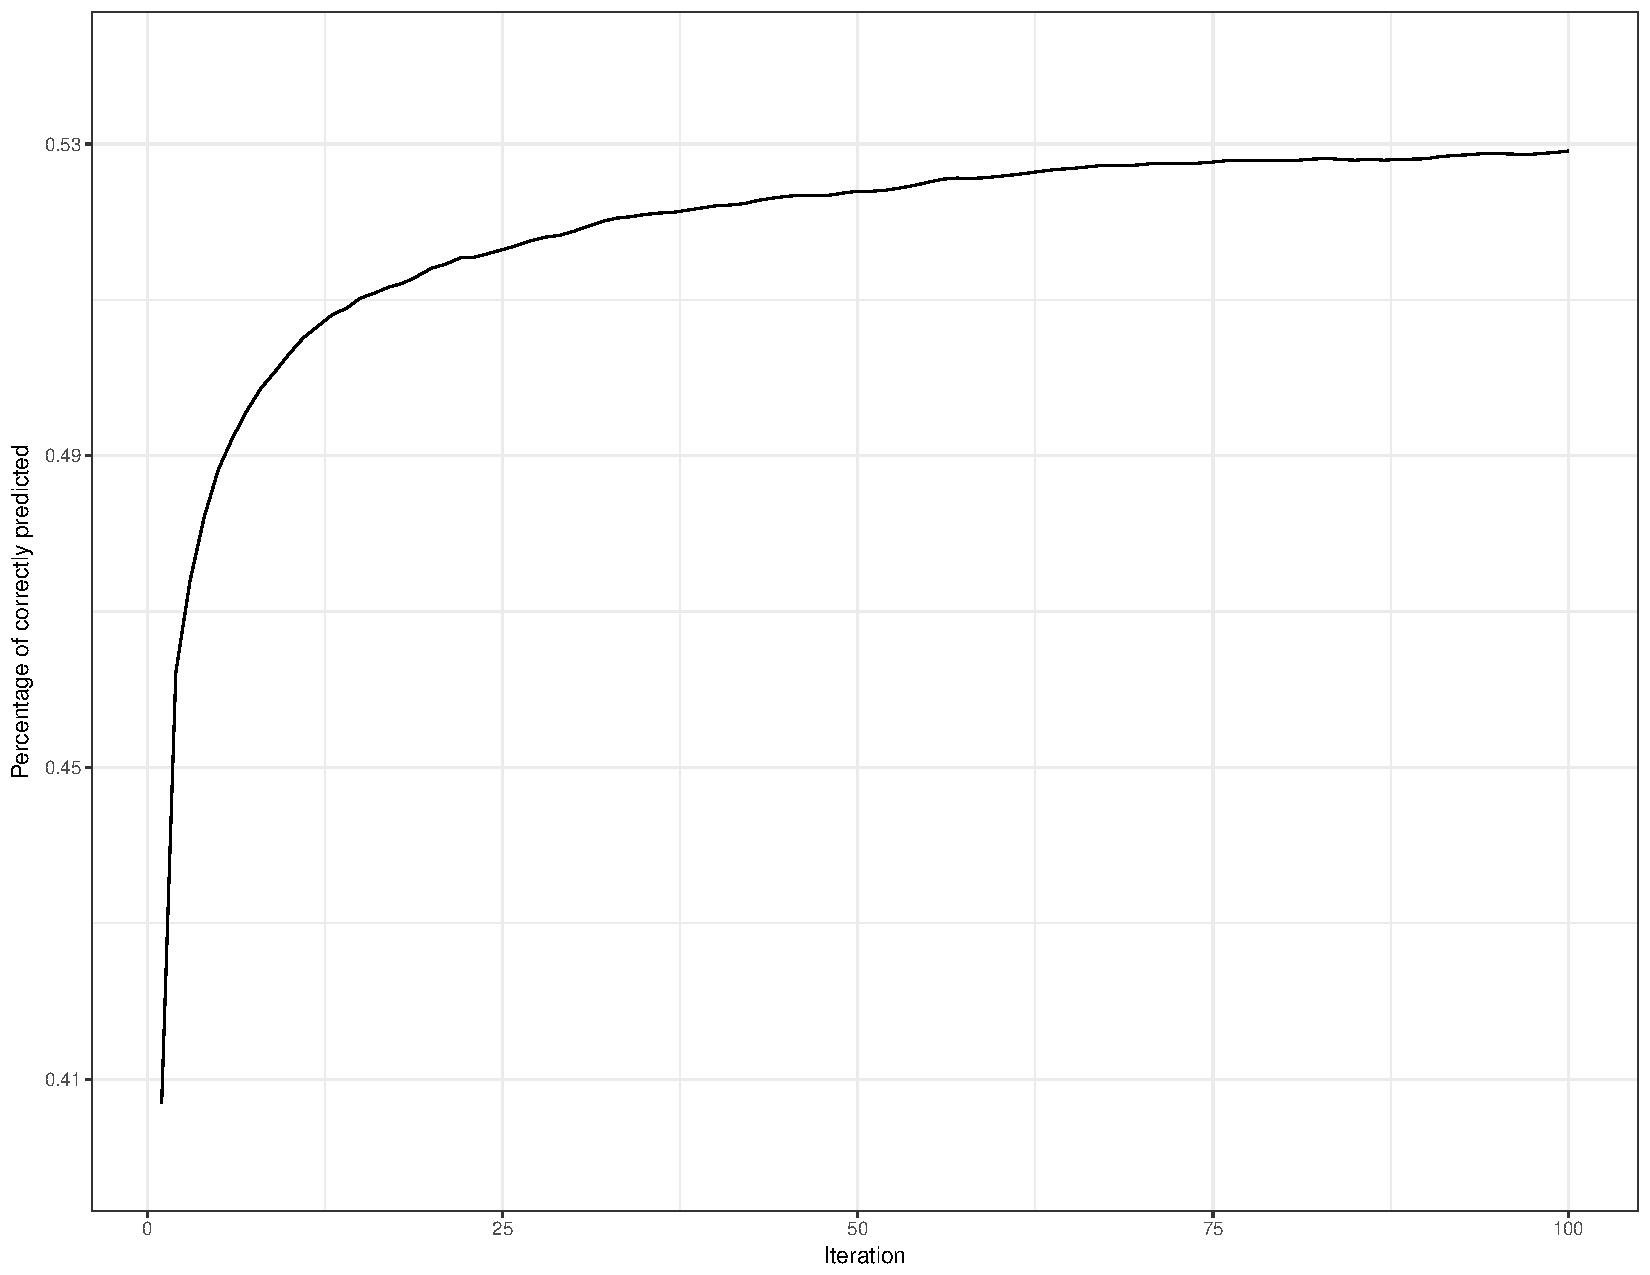
\includegraphics[width=0.8\textwidth]{figs/multiple_trainings}
\caption{Progress of prediction ability over multiple iterations}
\end{figure}

As shown in the graph, after the first iteration, the amount of randomly guessed outcomes has considerably lowered, which led to much better prediction ability. In the rest of the iterations, only slight improvements have been made, perhaps because of players with low number of matches played.

\subsection{Results}
In order to compare the quality of above-mentioned approaches, real soccer data have been evaluated with the intention of measuring the algorithms' ability to correctly predict future matches. Also, the log-likelihood loss is calculated as a different method of measurement. All approaches have been evaluated using both the logistic distribution used by chess players and normal distribution originally suggested by Arpad Elo.

Note that all values of prediction ability (PA) in \autoref{table:elo_results} are in percentage to provide a better picture about the ability.

Also, to provide a better perspective, it is worth noting that the state-of-the-art result of the prediction ability is around 53\% achieved by the bookkeepers. Results better than the state-of-the-art result are bold.

\begin{table}[H]
\caption{Prediction ability and log-likelihood loss of different approaches to Elo extensions}
\label{table:elo_results}
\centering
\begin{tabularx}{\textwidth}{ | l | X | X | X | X |}
\hline
& \multicolumn{2}{| c |}{\textbf{Logistic}} & \multicolumn{2}{| c |}{\textbf{Normal}} \\ \hline
& \textbf{PA} & \textbf{LL} &\textbf{PA} & \textbf{LL} \\ \hline
Treating teams as individuals & 44.59 & 0.638  & 44.23 & 0.634 \\ \hline
Pure extension & 46.22 & 0.615 & 44.03 & 0.621 \\ \hline
Parameter optimization & 46.54 & 0.615 & 44.21 & 0.620 \\ \hline
Overall rating & 46.50 & 0.613 & 44.41 & 0.619 \\ \hline
Ignoring draws & 51.64 & 0.615 & 51.58 & 0.621 \\ \hline
Bayes & \textbf{53.68} & 0.686 & 21.23 & 1.016 \\ \hline
PO \& OR \& Bayes & \textbf{53.72} & 0.691 & 21.02 & 1.042 \\ \hline
\end{tabularx}
\end{table}

\examplespace
\begin{example}
To provide an example of the extension for Elo, consider following lineups:

\begin{table}[H]
\centering
\begin{tabular}{l c c}
\textbf{Team} & \textbf{Player} & \textbf{Rating} \\
Team 1 ($T_1$) & Player A ($A$) & 1300 \\
& Player B ($B$) & 1400 \\
Team 2 ($T_2$) & Player C ($C$) & 1100 \\
& Player D ($D$) & 1000 \\
\end{tabular}
\end{table}

First of all, both $T_1$ and $T_2$ need to have the team rating calculated using \eqref{eq:obtaining_teams_rating}.

\begin{align*}
R_{T_1} &= \frac{1}{|T_1|}\sum_{R_j \in T_1}{R_j} \\
&= \frac{1}{2}(1300 + 1400) \\
&= 1350 \\[1.5em]
R_{T_2} &= \frac{1}{|T_2|}\sum_{R_j \in T_2}{R_j} \\
&= \frac{1}{2}(1100 + 1000) \\ 
&= 1050,
\end{align*}

\noindent obtaining ratings $R_{T_1} = 1350$ and $R_{T_2} = 1050$.

From here, the teams can be treated as individuals and therefore application of the expected score formula \eqref{eq:expected_score} produces expectancy of either team beating the other.

\begin{align*}
E_{T_1} &= \frac{1}{1+10^{\frac{R_{T_2} - R_{T_1}}{400}}} \\
&= \frac{1}{1+10^{-\frac{300}{400}}} \\
&\doteq 0.849 \\[1.5em]
E_{T_2} &= \frac{1}{1+10^{\frac{R_{T_1} - R_{T_2}}{400}}} \\
&= \frac{1}{1+10^{\frac{300}{400}}} \\
&\doteq 0.151,
\end{align*}

\noindent predicting that team $T_1$ will beat team $T_2$ with the probability of 0.849. This also makes intuitive sense if players' ratings of both teams are considered.
Say that team $T_2$ beat its odds and won the game. Considering $K$ factor of 32, this will affect the team ratings as follows.

\begin{align*}
R'_{T_1} &= R_{T_1} + K(S_{T_1} - E_{T_1}) \\
&= 1350 + 32(0 - 0.849) \\
&\doteq 1322.8 \\[1.5em]
R'_{T_2} &= R_{T_2} + K(S_{T_2} - E_{T_2}) \\
&= 1050 + 32(1 - 0.151) \\
&\doteq 1077.2,
\end{align*}

\noindent obtaining updated ratings $R'_{T_1} = 1322.8$ and $R'_{T_2} = 1077.2$.
Such ratings will then be propagated to the players $A$, $B$, $C$ and $D$. Propagation of the team rating to player $A$ is shown below while the procedure can be applied on other players analogously.

\begin{align*}
R'_A &= R_A + (R'_{T_1} - R_{T_1})\left(\frac{R'_{T_1} - (2S_{T_1} - 1)(R_A - R_{T_1})}{R'_{T_1}}\right) \\
&= 1300 + (1322.8 - 1350)\left(\frac{1322.8 - (0 - 1)(1300 - 1350)}{1322.8}\right) \\
&\doteq 1300 - 26.2 \\
& = 1273.8
\end{align*}

After applying the same procedure on other players, following table showing updated ratings of players and teams was produced.

\begin{table}[H]
\centering
\begin{tabular}{l c c c}
\textbf{Team} & \textbf{Team rating} & \textbf{Player} & \textbf{Player rating} \\
Team 1 ($T_1$) & 1322.83 & Player A ($A$) & 1273.86 \\
& & Player B ($B$) & 1371.80 \\
Team 2 ($T_2$) & 1077.17 & Player C ($C$) & 1125.91 \\
& & Player D ($D$) & 1028.54
\end{tabular}
\end{table}
\end{example}
\chapter{Batch ranking algorithms}
\label{ch:batch_ranking}
In contrary to online ranking algorithms, \textbf{batch ranking algorithms} do not represent player's rating in a single state, but they take in account outcomes of all previous matches in order to establish a leader board.

Although this may seem like a more thorough way to go, processing all previous matches is more computationally complex and may be too computationally difficult for bigger datasets.

\section{Graph-based ranking}
\label{sec:pagerank}
A famous representant of a graph-based ranking system is Google's PageRank introduced by \citet{PagePageRankcitationranking1998} to rank importance of web pages in Google Search Engine. The core idea is that the importance of a page should be based on the number and importance of pages that point to the page. Such idea can be expressed using a recursive formula.

\begin{equation}
r(P) = \sum_{Q \in B_P} \frac{r(Q)}{|Q|},
\label{eq:pagerank}
\end{equation}

\noindent where $r(x)$ is the rating of page $x$, $Q \in B_P$ is the set of all pages $Q$ pointing to page $P$ and $|Q|$ is the number of pages Q is pointing to. This shows that the more pages a page points to, the more the page lowers its effect on the importance of these pages and therefore the importance of a page can be viewed as number of \textit{votes} the page can \textit{vote} in favor of other pages.

All of the pages indexed by Google create a directed graph of pages pointing to each other. Since the PageRank formula \eqref{eq:pagerank} is recursive, the nodes of the graph are initialized at the same value and then the PageRank of each node is iteratively updated until the value of PageRank converges. This can be expressed as follows.

\begin{equation*}
r_{i+1}(P) = \sum_{Q \in B_P} \frac{r_i(Q)}{|Q|} ,\quad i = 0, 1, 2, \dots,
\end{equation*}

\noindent where $r_{i+1}(P)$ is the rating of page P in iteration $i+1$, while $r_i(Q)$ is the rating of page Q in iteration $i$.

\subsection{Adapting PageRank to soccer}
As \citet{LazovaPageRankApproachRanking2015} explain, in order to adapt PageRank algorithm to soccer games, nodes of the graph represent teams instead of pages. An edge exists between all nodes that represent teams that have played a match against each other. Note that in difference to the PageRank's original graph, teams always have an edge in both directions. The values of the edges are calculated by a function that can take into account any information about the teams' relations (win/lose ratio, goals scored, number of draws, \dots).

Let matrix $A$ be the adjacency matrix of said graph. As \citet{GOVANRANKINGNATIONALFOOTBALL} explain, in order to ensure the convergence of PageRank algorithm, a matrix $Q$ is derived from A as follows.

\begin{align}
\label{eq:a_to_q}
Q_{i,j} = (1-d)\cdot \frac{A_{i,j}}{\sum_{k=1}^{N} A_{i,k}} + \frac{d}{N}
\end{align}

\noindent with $A_{i,j}$ representing $i$-th row and $j$-th column of the matrix A and $N$ representing number of teams.

Similarily to the original PageRank algorithm, the PageRank value of each team is calculated by the iterative process. After the ratings have converged, teams ratings will be represented by a value from the interval $(0, 1)$ with greater values expressing the team is stronger.

\examplespace
\begin{example}
To obtain a better understanding of PageRank, let's rank four teams A, B, C and D that have played following matches:\\[0.5em]
\begin{tabular}{l c r} 
A & 3:1 & B \\
A & 2:1 & C \\
B & 1:1 & C \\
B & 2:0 & D \\
\end{tabular}\\[0.5em]
meaning that A has won three matches against B and lost one, B has defeated C in two matches and have not lost a single match, etc.
For simplicity, we will disregard number of goals scored.

For a better visualization of the match-ups, a bidirectional graph can be constructed. Note that the weight of the edges denotes how many \textit{votes} does a team give in favor of the other team, therefore for teams A and B, the weight of edge from A to B is 1 and 3 for the edge from B to A.

\vspace{1em}
\begin{figure}[H]
\centering
\begin{tikzpicture}
  \SetGraphUnit{3}
  \Vertex{B}
  \NOWE(B){A}
  \SOWE(B){C}
  \EA(B){D}
  \Edge[label = 1](A)(B)
  \Edge[label = 1](B)(C)
  \Edge[label = 1](A)(C)
  \Edge[label = 0](B)(D)
  \tikzset{EdgeStyle/.append style = {bend left = 50}}
  \Edge[label = 2](C)(A)
  \tikzset{EdgeStyle/.append style = {bend right = 50}}
  \Edge[label = 2](D)(B)
  \Edge[label = 3](B)(A)  
  \Edge[label = 1](C)(B)
\end{tikzpicture}
\end{figure}

A weighting function has to be applied to achieve proper values of the edges. For simplicity of the example, following function is applied.

\begin{equation*}
f_{i,j} = \frac{w_{i,j}}{g_{i,j}},
\end{equation*}

\noindent where $f_{i,j}$ is the calculated weight between nodes $i$ and $j$, $w_{i,j}$ is number of matches won by $i$ against $j$ and $g_{i,j}$ is number of total games played between $i$ and $j$. After applying such function on every edge, the graph looks as follows. Also, this introduces the \textit{damping factor} $d$, which adds some randomness to the procedure. This ensures that the iterative procedure will eventually converge. Also, the damping factor is somewhat intuitive, because it adds a small winning probability for teams that have never played against each other. The damping factor is user-defined and the authors of PageRank suggest using conservative value of 0.15.

Then, the PageRanks are assigned initial values and the algorithm iterates until the values converge. In every iteration, following equation is executed, leading to the change in PageRank values.

\begin{equation*}
\pi_{t+1}^T = \pi_t^TQ,\quad t= 0, 1, 2, \dots,
\end{equation*}

with $t$ representing current iteration and $\pi_t$ vector of PageRanks in current iteration. Note that $\pi_0$ can be chosen either randomly or homogeneously.

\vspace{1em}
\begin{figure}[H]
\centering
\begin{tikzpicture}
  \SetGraphUnit{3}
  \Vertex{B}
  \NOWE(B){A}
  \SOWE(B){C}
  \EA(B){D}
  \Edge[label = $\frac{1}{4}$](A)(B)
  \Edge[label = $\frac{1}{2}$](B)(C)
  \Edge[label = $\frac{1}{3}$](A)(C)
  \Edge[label = 0](B)(D)
  \tikzset{EdgeStyle/.append style = {bend left = 50}}
  \Edge[label = $\frac{2}{3}$](C)(A)
  \tikzset{EdgeStyle/.append style = {bend right = 50}}
  \Edge[label = 1](D)(B)
  \Edge[label = $\frac{3}{4}$](B)(A)  
  \Edge[label = $\frac{1}{2}$](C)(B)
\end{tikzpicture}
\end{figure}

\noindent which corresponds to following adjacency matrix.

\[
\renewcommand\arraystretch{1.5}
A = 
\begin{bmatrix}
0 & \frac{1}{4} & \frac{1}{3} & 0 \\
\frac{3}{4} & 0 & \frac{1}{2} & 0 \\
\frac{2}{3} & \frac{1}{2} & 0 & 0 \\
0 & 1 & 0 &0
\end{bmatrix}
\]  

In the next step, the adjacency matrix A is converted to matrix Q using formula \eqref{eq:a_to_q}. For the sake of easier calculation, we have chosen the damping factor $d = \frac{1}{5}$ for this example, hence the matrix Q:

\[
\renewcommand\arraystretch{1.5}
Q = 
\begin{bmatrix}
\frac{1}{20} & \frac{55}{140} & \frac{71}{140} & \frac{1}{20} \\
\frac{53}{100} & \frac{1}{20} & \frac{37}{100} & \frac{1}{20} \\
\frac{71}{140} & \frac{55}{140} & \frac{1}{20} & \frac{1}{20} \\
\frac{1}{20} & \frac{17}{20} & \frac{1}{20} & \frac{1}{20}
\end{bmatrix}
\]

Now, a vector of teams' PageRank values $\pi_0^T$ is created. This vector is then iteratively multiplied with the matrix Q until the values converge. We can conservatively initialize the PageRank values to the same value for every team:

\begin{equation*}
\pi_0^T = 
\begin{bmatrix}
\frac{1}{4} & \frac{1}{4} & \frac{1}{4} & \frac{1}{4}
\end{bmatrix}
\end{equation*}

Finally, the iterative procedure starts. For this example, one iteration of the procedure is calculated:

\begin{equation*}
\pi_{t+1}^T = \pi_t^TQ,\quad t= 0, 1, 2, \dots
\end{equation*}

Therefore, the first iteration of our example is calculated as follows.

\begin{align*}
\pi_1^T &= 
\begin{bmatrix}
\frac{1}{4} & \frac{1}{4} & \frac{1}{4} & \frac{1}{4}
\end{bmatrix} 
\cdot
\begin{bmatrix}[1.5]
\frac{1}{20} & \frac{55}{140} & \frac{71}{140} & \frac{1}{20} \\
\frac{53}{100} & \frac{1}{20} & \frac{37}{100} & \frac{1}{20} \\
\frac{71}{140} & \frac{55}{140} & \frac{1}{20} & \frac{1}{20} \\
\frac{1}{20} & \frac{17}{20} & \frac{1}{20} & \frac{1}{20}
\end{bmatrix} \\[1em]
&= 
\begin{bmatrix}
\frac{859}{3200} & \frac{59}{115} & \frac{171}{700} & \frac{1}{20}
\end{bmatrix}
\end{align*}

The vector $\pi_1^T$ holds the teams' PageRanks after first iteration. In order to calculate next iteration's result, the same matrix Q is multiplied with $\pi_1^T$ obtained in the first iteration.

After the algorithm converges, the values in $\pi$ are teams' final PageRanks. Higher PageRank of a team means that the team is considered to be better. Therefore, in this example after the first iteration, player B is considered to be the best one, A the second, C the third and D is the worst.
\end{example}

\subsection{Cons of PageRank}
While other ranking algorithms usually perceive team as a set of individuals, PageRank perceives a team as a blackbox. This leads to lack of knowledge about individual players, which makes for the disability of examining players' skill individually. Also, changes in team's structure are not projected to the team's PageRank rating, which is a solid property for building leader boards, but it causes difficulties in matching teams with equally strong opponents.

\subsection{Applying graph-based ranking on real data}
Using the PageRank algorithm adapted for soccer games, an empty oriented graph with nodes representing teams is created and fit with appropriate data. After the graph is created, the edges are assigned weights using functions listed below. 

\vspace{1em}
\begin{tabular}{l}
$f_{i,j} = \frac{\ell_{i,j}}{g_{i,j}}\cdot \frac{1}{G-g_{i,j}+1}$\\[1em]
$f_{i,j} = \frac{\ell_{i,j}}{g_{i,j}}$\\[1em]
$f_{i,j} = \frac{\ell_{i,j}}{g_{i,j}} + \frac{c_{i,j}}{c_{i,j}+s_{i,j}}$\\[1em]
$f_{i,j} = \ell_{i,j}$\\[1em]
$f_{i,j} = \frac{c_{i,j}}{s_{i,j}}$\\[1em]
$f_{i,j} = \frac{\ell_{i,j}}{w_{i,j}}$\\[1em]
$f_{i,j} = \frac{\ell_{i,j}}{g_{i,j}}+0.5\cdot \frac{d_{i,j}}{g_{i,j}}$\\[1em]
$f_{i,j} = \frac{c_{i,j}}{c_{i,j}+s_{i,j}}$\\[1em]
$f_{i,j} = \frac{c_{i,j}}{g_{i,j}}$\\[1em]
$f_{i,j} = c_{i,j}$
\end{tabular}
\vspace{1em}

\noindent where\\

\vspace{-1.2em}
\begin{table}[H]
\begin{tabular}{rl}
$f_{i,j}$\quad &is the weight of edge from $i$ to $j$,\\
$g_{i,j}$\quad &is the number of games played between $i$ and $j$,\\
$\ell_{i,j}$\quad &is the number of games $i$ lost against $j$,\\
$w_{i,j}$\quad &is the number of games $i$ won against $j$,\\
$d_{i,j}$\quad &is the number of games drawn between $i$ and $j$,\\
$c_{i,j}$\quad &is the number of goals $j$ has scored in all matches against $i$,\\
$s_{i,j}$\quad &is the number of goals $i$ has scored in all matches against $j$,\\
$G$\quad &is the maximum number of games played between any two teams
\end{tabular}
\end{table}
\vspace{-1em}

After determining the weights of the graph, the graph is represented as a matrix and the PageRank iterative procedure calculates appropriate PageRank of every function used. The goal is to detect such function that will be most successful in predicting outcomes of given matches. To calculate the belief in a team's victory, Bradley-Terry model with given team's PageRank $\pi_A$ as his score, hence \eqref{eq:pagerank_bradley_terry}.

\begin{equation}
\label{eq:pagerank_bradley_terry}
P(A > B) = \frac{\pi_A}{\pi_A + \pi_B}
\end{equation}

Following such principle for every PageRank's weighting function, results as shown in \autoref{table:pagerank_results} were obtained.

\vspace{1em}
\begin{table}[H]
\caption{Results of different weighting functions used with the extended PageRank algorithm}
\label{table:pagerank_results}
\begin{tabular}{| l | r | r |}
\hline
\textbf{Function} & \textbf{Matches predicted} & \textbf{Log-likelihood loss} \\ \hline
$\frac{\ell_{i,j}}{g_{i,j}}\cdot \frac{1}{G-g_{i,j}+1}$ &  36.55 & 0.695 \\ \hline
$\frac{\ell_{i,j}}{g_{i,j}}$ &  38.34 & 0.679 \\ \hline
$\frac{\ell_{i,j}}{g_{i,j}} + \frac{c_{i,j}}{c_{i,j}+s_{i,j}}$ &  36.06 & 0.684 \\ \hline
$\ell_{i,j}$ &  34.82 & 0.722 \\ \hline
$\frac{c_{i,j}}{s_{i,j}}$ &  37.14 & 0.679 \\ \hline
$\frac{\ell_{i,j}}{w_{i,j}}$ &  37.90 & 0.713 \\ \hline
$\frac{\ell_{i,j}}{g_{i,j}}+0.5\cdot \frac{d_{i,j}}{g_{i,j}}$ &  36.46 & 0.683 \\ \hline
$\frac{c_{i,j}}{c_{i,j}+s_{i,j}}$ &  34.79 & 0.690 \\ \hline
$\frac{c_{i,j}}{g_{i,j}}$ &  34.77 & 0.694 \\ \hline
$c_{i,j}$ & 31.49 & 0.750 \\ \hline
\end{tabular}
\end{table}

\section{Supervised Learning approach to match prediction}
Supervised Learning is a machine learning task of approximating a function based on known input-output pairs. Such input-output pairs consist of an input vector, which represents the argument to the approximated function, and an output vector, which holds the output of the function. The Supervised Learning algorithm analyzes the training data in order to create a function that can then be used to calculate outputs. In other words, Supervised Learning is an algorithm solving a regression task.

Numerous approaches to Supervised Learning exist, from simpler ones like Linear or Logistic Regression, to more complicated ones like Support Vector Machines or Neural Networks. For the task of predicting outcomes of soccer matches, we have decided to use Multilayer Perceptron, which is a feedforward artificial Neural Network.

The Multilayer Perceptron has been chosen as the Supervised Learning algorithm due to recent popularity of Neural Networks, as well as their capability of approximating any function, if the right network structure is used. This is shown has been shown by \citet{HornikApproximationCapabilitiesMultilayer1991} and is known as the Universal approximation theorem.

\subsection{Perceptron}
Simple Perceptron introduced by \citet{RosenblattPerceptronProbabilisticModel1958} is an algorithm for Supervised Learning that is able to classify linearly separable set of data. It often represents a single neuron in a Neural Network and it can be visualized as shown in figure \ref{fig:perceptron_tikz}.

\vspace{1em}
\begin{figure}[H]
\caption{Perceptron}
\label{fig:perceptron_tikz}
\centering
\begin{tikzpicture}
  % Vertices
  \node[vertex] (x1) at (0,3)  {$x_1$};
  \node[weights] (w1) at (1.5,3) {$w_1$};
  \node[vertex] (x2) at (0,2)  {$x_2$};
  \node[weights] (w2) at (1.5,2) {$w_2$};
  \node[vertex] (xn) at (0, 0) {$x_n$};
  \node[weights] (wn) at (1.5,0) {$w_n$};
  \node[vertex] (f) at (4, 1.5) {$\mathlarger{\sum}$};
  \node[vertex] (b) at (4, 0) {$\theta$};
  \node[vertex, text width=2.5em] (step) at (6, 1.5) {};
  \node[vertex] (y) at (8, 1.5) {$y$};
  
  % Comments
  \node[note] (x_note) at (0, -0.8) {Inputs};
  \node[note] (w_note) at (1.5, -0.8) {Weights};
  \node[note] (b_note) at (4, -0.7) {Bias};  
  \node[note, text width=4em, text centered] (activation_note) at (6, 0.3) {Activation function};  
  \node[note] (y_note) at (8, 0.8) {Output};  
  
  % Dots between x_2 and x_n
  \node[below of=x2] (dots) {$\vdots$};
  \node[below of=w2] (dots) {$\vdots$};

  % Edges
  \draw (x1) edge [->, draw=black!50] (w1);
  \draw (x2) edge [->, draw=black!50] (w2);
  \draw (xn) edge [->, draw=black!50] (wn);
  \draw (w1) edge [->, draw=black!50] (f);
  \draw (w2) edge [->, draw=black!50] (f);
  \draw (wn) edge [->, draw=black!50] (f);
  \draw (step) edge [->, draw=black!50] (y);
  \draw (f) edge [->, draw=black!50] (step);
  \draw[dashed] (b) edge [->, draw=black!50] (f);
  
  % Step function
  \draw[ultra thick] (5.7,1.3) -- (6,1.3) -- (6,1.8) -- (6.3,1.8);
  \draw (6,1.1) -- (6,1.9);
  \draw (5.6,1.5) -- (6.4,1.5);
\end{tikzpicture}
\end{figure}

In the figure, $(x_1, x_2, \cdots, x_n)$ represents the vector of inputs with appropriate weights $(w_1, w_2, \cdots, w_3)$. Another important feature is the $\theta$, which represents threshold of the Perceptron. This can be expressed mathematically as

\begin{align*}
\sum_{i=1}^{n}{x_i\cdot w_i} \geq \theta.
\end{align*}

The threshold can also be perceived as an additional input with weight of 1, creating vectors of inputs and appropriate weights $(-\theta, x_1, x_2, \cdots, x_n)$ and $(1, w_1, w_2, \cdots, w_n)$, respectively. The product of such two vectors $\xi$ is called \textit{potential} and is passed as an argument to an activation function, which outputs the actual result of the Perceptron. Therefore, the output of the Perceptron can be expressed as

\begin{align*}
y = f\left(\sum_{i=0}^{n}{x_i\cdot w_i}\right),
\end{align*}

\noindent where $f(\cdot)$ is the activation function.

There are numerous activation function that can be used, from which an example of few is provided.
\begin{itemize}
\item Binary step: $$y = \begin{cases}1 & if \sum\limits_{i=0}^{n}{x_i\cdot w_i} \geq 0 \\ 0 & if \sum\limits_{i=0}^{n}{x_i\cdot w_i} < 0,\end{cases}$$
\item Logistic: $$f(\xi) = \frac{1}{1+e^{-\xi}}, \qquad \xi = \sum_{i=0}^{n}{x_i\cdot w_i},$$
\item Gaussian: $$f(\xi) = e^{-\xi^2}, \qquad \xi = \sum_{i=0}^{n}{x_i\cdot w_i}.$$
\end{itemize}

After the output si known, the Perceptron compares the actual output with the presented output and adjusts the weights accordingly. Input samples are presented to the algorithm until it converges and separates the data. Note that as \citet{NovikoffConvergenceProofsPerceptrons1962} stated, the convergence of the Perceptron is certain.

Then the Perceptron is considered trained and new inputs can be presented to predict their output based on the separation of the data.

\subsection{Multilayer Perceptron}
\label{sec:multilayer_perceptron}
Unfortunately, the Perceptron's ability in separating data is limited. It often happens that the separation is not sufficient and multiple Perceptrons have to be used in multiple layers in order to achieve more precise data separation, creating a Multilayer Perceptron of $n \geq 2$ layers. In such $n$ layers, there is always one input layer with $m = |x|$ neurons, every neuron accepting one element of the input vector $x$. The input layers is fully connected to $n-2$ hidden layers with no strict restriction on number of neurons. Also, every $i$-th hidden layer is fully connected to $(i+1)$-th layer. Finally, the last layer is the output layer, presenting outputs of given inputs, also fully connected to the last hidden layer. This can be visualized as follows.

\vspace{1em}
\begin{figure}[H]
\caption{Multilayer Perceptron}
\centering
\begin{tikzpicture}[shorten >=1pt,->,draw=black!50, node distance=\layersep]
    \tikzstyle{every pin edge}=[<-,shorten <=1pt]
    \tikzstyle{annot} = [text width=4em, text centered]

    % Draw the input layer nodes
    \foreach \name / \y in {1,...,2}
    % This is the same as writing \foreach \name / \y in {1/1,2/2,3/3,4/4}
        \node[vertex] (I-\name) at (0,-\y) {$x_\y$};
    \node[vertex] (I-3) at (0,-4) {$x_n$};

    % Draw the hidden layer nodes
    \foreach \name / \y in {1,...,5}
        \path[yshift=0.5cm]
            node[vertex, text width=1.2em] (H-\name) at (\layersep,-\y cm) {};

    % Draw the output layer node
    \node[vertex, pin={[pin edge={->}]right:Output}, right of=H-3] (O) {$y$};

    % Connect every node in the input layer with every node in the
    % hidden layer.
    \foreach \source in {1,...,3}
        \foreach \dest in {1,...,5}
            \path (I-\source) edge (H-\dest);

    % Connect every node in the hidden layer with the output layer
    \foreach \source in {1,...,5}
        \path (H-\source) edge (O);

    % Annotate the layers
    \node[annot,above of=H-1, node distance=1cm] (hl) {Hidden layer};
    \node[annot,left of=hl] {Input layer};
    \node[annot,right of=hl] {Output layer};
    
     \node[] at(0,-3) (dots) {$\vdots$};
\end{tikzpicture}
\end{figure}

As the figure implies, every edge represents a weight and every node a neuron with appropriate value. The neuron's value is calculated similarly as in the Perceptron as a product of inputs and weights. Note that every layer has its own threshold value. 
After the output is determined, an error with respect to the presented output is calculated and the weights are modified accordingly. One of the algorithms used to modify the weights accordingly to the error is the backpropagation algorithm \citep{RumelhartNeurocomputingFoundationsResearch1988}. After the weights are modified, the algorithm iteratively presents inputs to the network until the error of the network $E$ is smaller than a predefined value. The error $E$ is calculated as

\begin{align*}
E = \frac{1}{2}\sum_{p}\sum_{o}(y_{o,p} - d_{o,p})^2,
\end{align*}

\noindent where $p$ is the set of all patterns, $o$ is the vector of output neurons and $y_{o,p}$ and $d_{o,p}$ are the calculated and desired outputs of input $p$ on output neuron $o$, respectively. This is called the mean squared error and is merely one of the functions that can be used to calculate the error.

After the network converges, new inputs can be presented to obtain a regression of outputs.

\subsection{Applying MLP on soccer data}
The Multilayer Perceptron can be applied on soccer data by presenting known matches with their outcomes to the network and obtaining predictions of unknown matches.

\subsubsection{Data preprocessing}
In order to achieve more accurate predictions, preprocessing of the data is required. The input data are presented as a vector of all players, while $1$ represents a player that belongs to the home team in given match, $-1$ a player that played in the away team and $0$ if the player have not played in the particular match. The outputs are based on goal difference in the particular match between $i$-th and $j$-th team and are calculated as

\begin{align*}
y = \frac{s_i}{s_i + s_j},
\end{align*}

\noindent with $s$ representing the goals scored by given team.

\examplespace
\begin{example}
To provide a better understanding of how soccer data are presented to the network, consider a match between team $i$ of players $A, C$ and team $j$ of players $D$ and $F$. Also, consider that team $i$ has won the game by scoring 3 goals in contrary to team $j$, which scored $1$ goal, and that players $B$ and $E$ have not taken place in the match. Then the input vector would be presented to the network as

\begin{align*}
x = \begin{bmatrix}
1 & 0 & 1 & -1 & 0 & -1
\end{bmatrix}
\end{align*}

\noindent where $x_1$ would be presented to the first input neuron, $x_2$ to the second, \dots

The output vector would be

\begin{align*}
y = \begin{bmatrix}
\frac{3}{4}
\end{bmatrix}.
\end{align*}
\end{example}

\subsubsection{Network structure}
In the process of predicting matches, the network structure is significantly influential. There are many parameters that can be set differently and every settings produces a slightly different results. Here are the parameters we have used for outcome predictions:

\begin{itemize}
\item \textbf{Activation function} decides what the output value of a neuron is. Since the soccer predictions represent probabilities of a team's victory, it is desired for the activation function's output to be from the interval $[0, 1]$. Therefore, we have used the softmax activation function, which is a generalization of the logistic function frequently used throughout this thesis. On the hidden layers, linear function is used, making the output reflect the input.

\item \textbf{Loss function} calculates the error of the network. In the description of MLP, mean squared error was mentioned as a loss function. This is, however, optional and different functions can be used. For soccer games, categorical cross entropy function was used, as it produces lower errors than mean squared error function if the matches are closer to its presented category.

\item \textbf{Optimizer} is an algorithm that helps the network find the appropriate weights faster. For purpose of predicting soccer games, the RMSProp algorithm is used, which modifies the learning rate (i.e. how significantly are the weights updated) with respect to the function's gradient. In contrary to AdaGrad algorithm, which is the algorithm RMSProp is based upon, it gives smaller significance to gradients calculated in previous iterations.

\item \textbf{Number of epochs} determines how many iterations of the whole dataset should be used to train the network. For the match predictions, multiple choices of number of epochs were used, although greater numbers led to worse final predictions. 

\item \textbf{Batch size} establishes how many inputs should be processed before adjusting the weights based on the error. Note that higher numbers generally lead to smaller significance of outliers while lower numbers lead to more frequent update of the weights and therefore bigger chance of finding appropriate result sooner. Again, multiple choices were tested on the network, usually achieving better results with lower values.

\item \textbf{Number of layers and neurons} decides how many hidden layers should be used with how many neurons. This is most certainly a tricky attribute and no direct instruction on how many layers to use when exists. Multiple options were tried, leading to a conclusion that one hidden layer with ten neurons produces sufficient results. Note that with increasing number of layers and neurons, the computational complexity increases excessively.
\end{itemize}

\subsection{Results}
Using Multilayer Perceptron for predicting outcomes of matches, solid prediction ability of \textasciitilde 45\% was achieved. However, the result can vary a lot by current structure of the network and parameter settings. 

It is also important to note that the error on training data has decreased throughout epochs, while error on validation data has increased as shown in \ref{fig:overfitting}. This is an indicator of overfitting \citep{CaruanaOverfittingNeuralNets2000}.

\begin{figure}[H]
\caption{Comparison of training and validation loss}
\label{fig:overfitting}
\centering
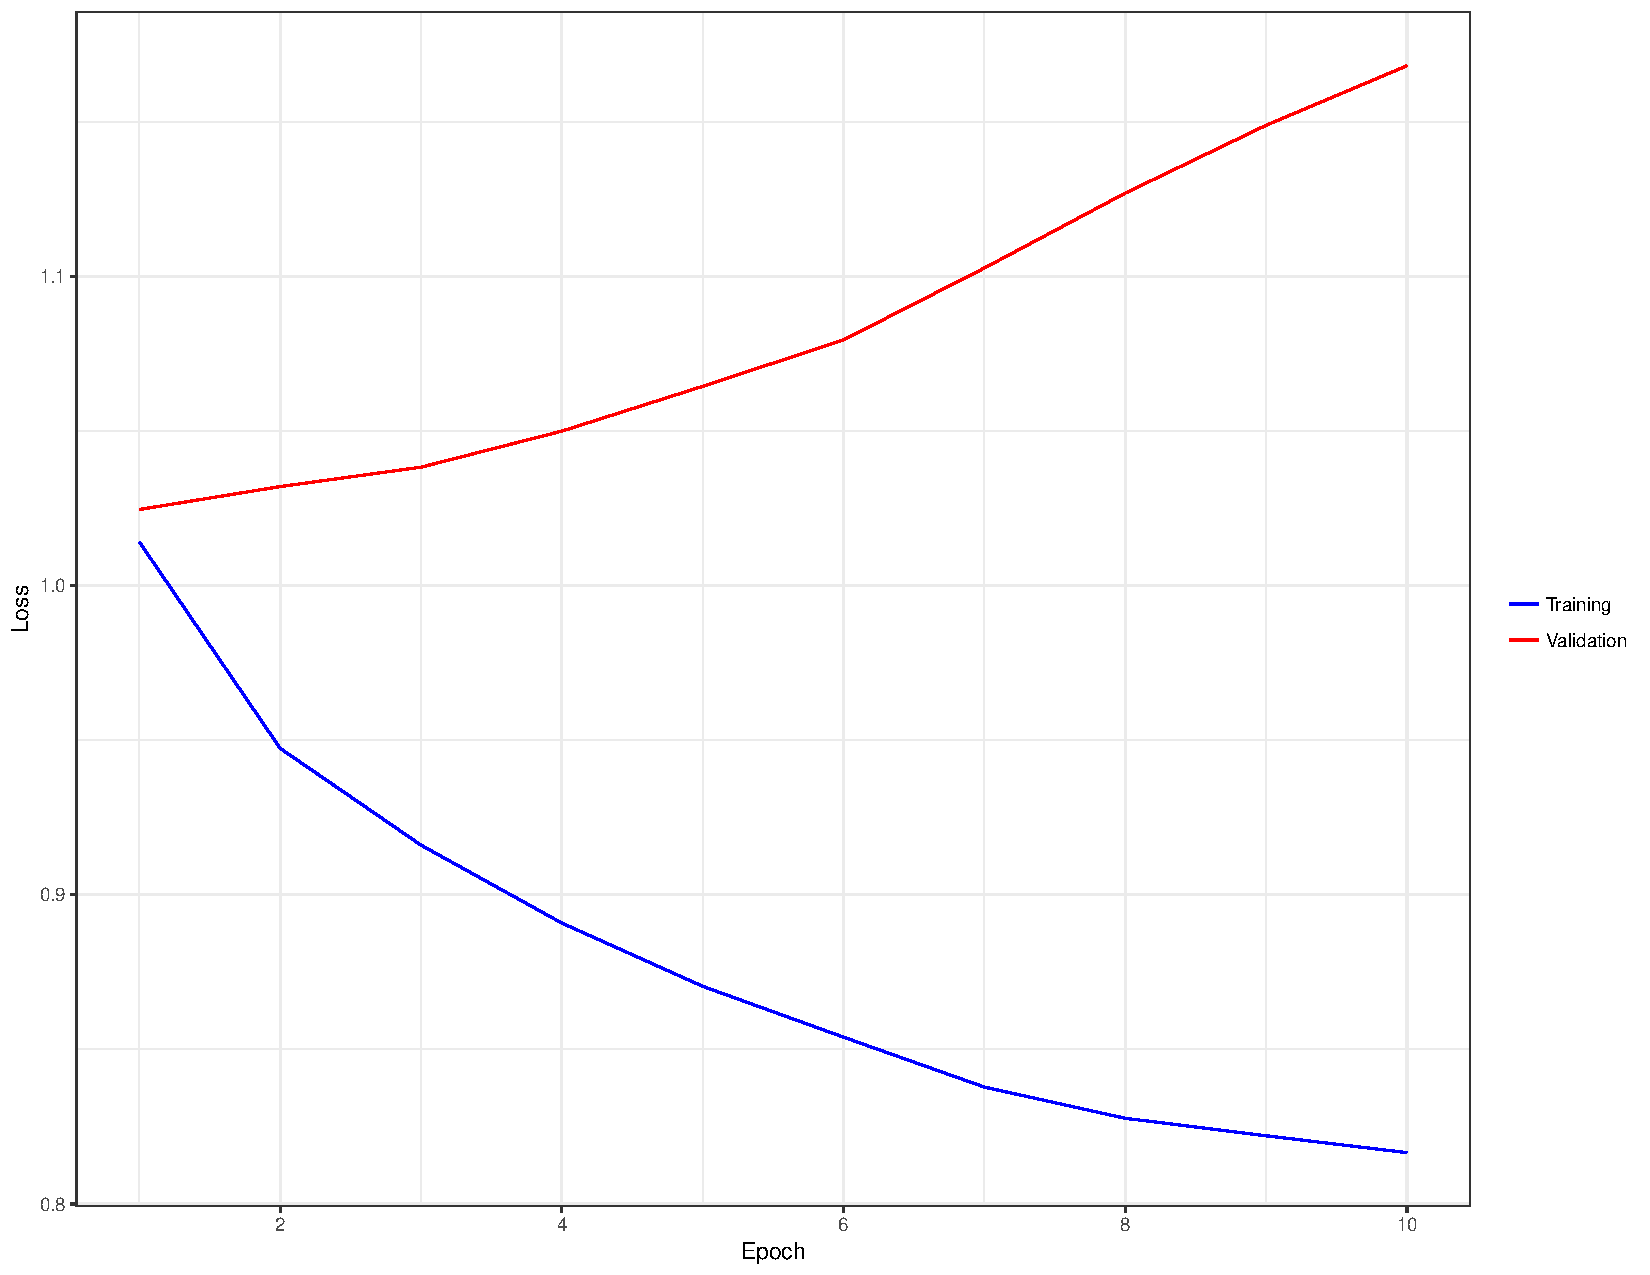
\includegraphics[width=0.8\textwidth]{figs/overfitting}
\end{figure}

Overfitting is believed to happen, among other cases, when the number of trainable parameters is too high compared to the number of data points. In the case of predicting soccer matches, we have 10787 input neurons, each neuron representing a player's relation to given match, and 21373 data points, each representing a match. That is, perhaps, insufficient number of matches given the number of players and therefore, the overfitting problem could be solved by introducing more matches to the network. However, since more data is not available, a method called dropout \citep{SrivastavaDropoutSimpleWay2014} helping to overcome ovefitting has been introduced to the hidden layer. Dropout determines the probability of ignoring a certain neuron and therefore precludes overfitting. By using a dropout probability of 0.4, much better results were achieved as the prediction ability increased to \textasciitilde 49\% and the validation loss was somewhat constant throughout the epochs.

\begin{figure}[H]
\caption{Comparison of training and validation loss with dropout}
\centering
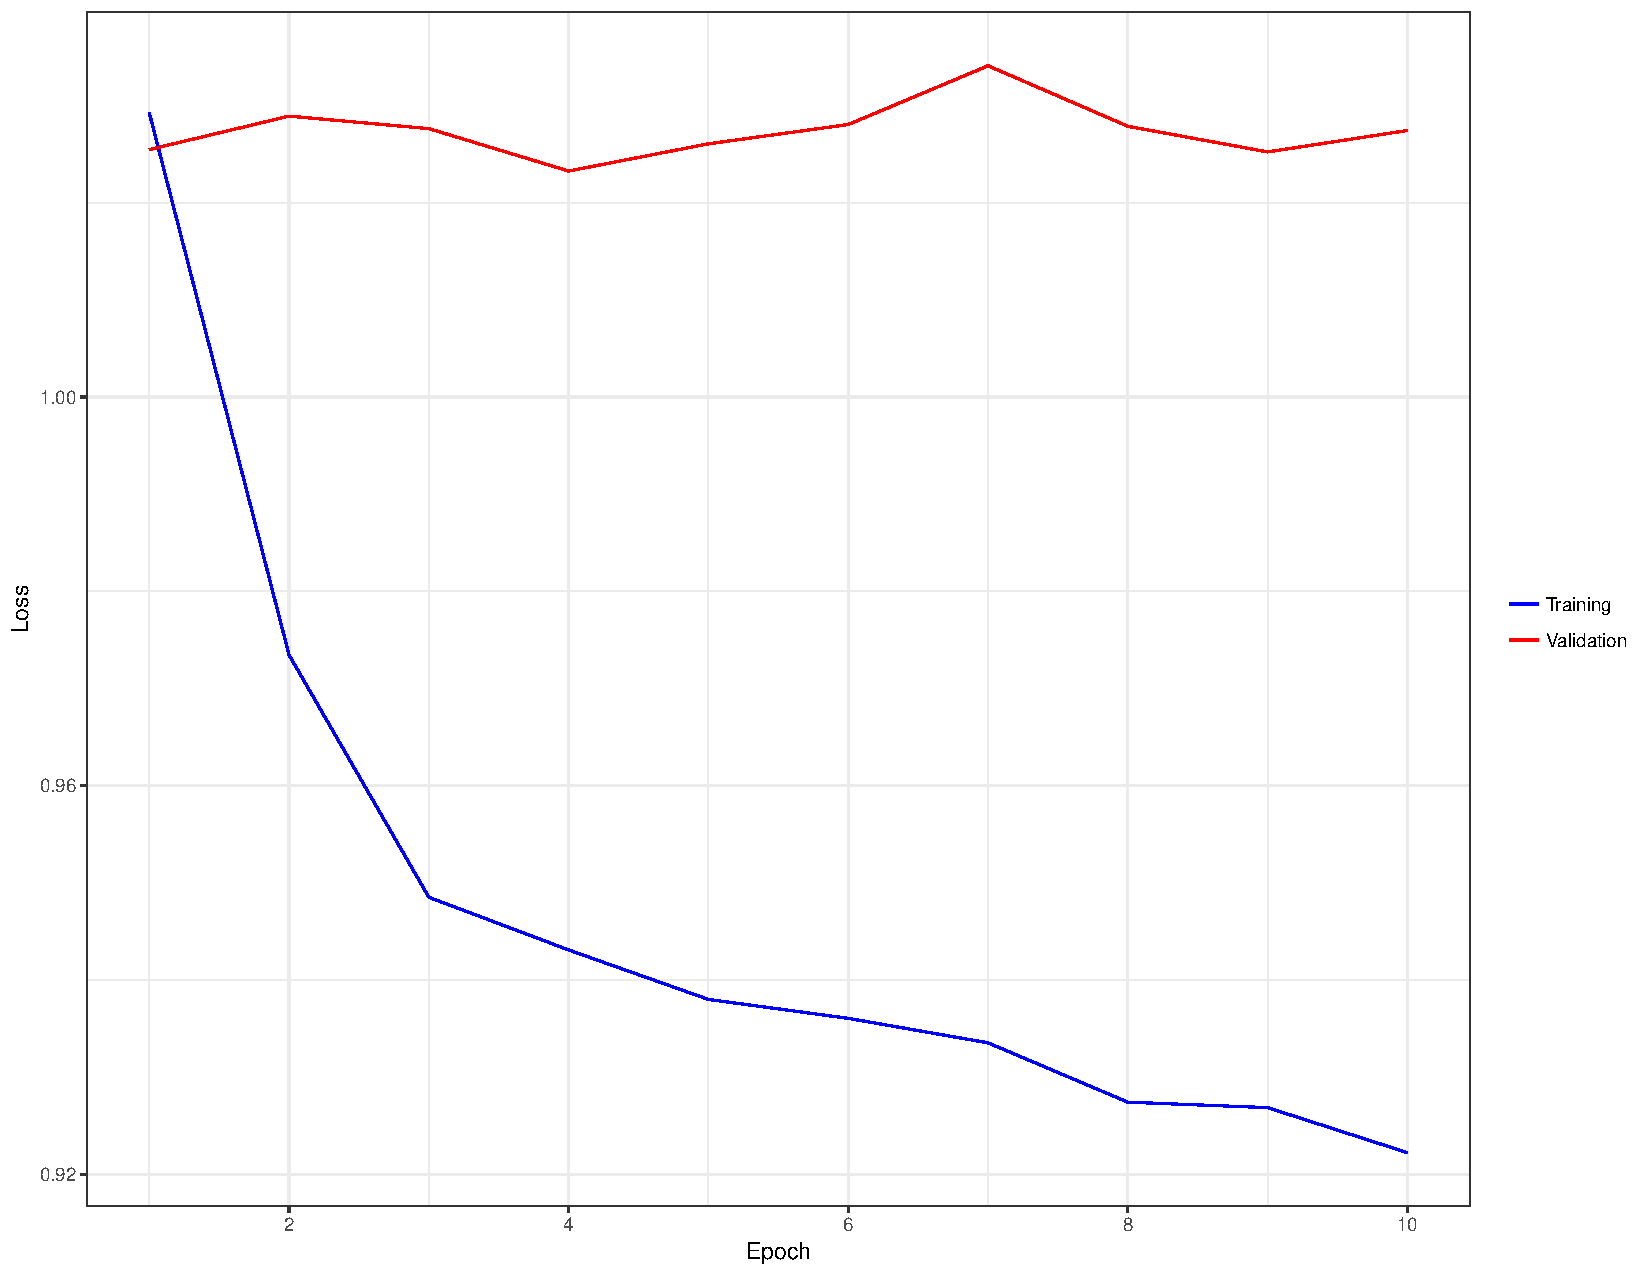
\includegraphics[width=0.8\textwidth]{figs/overfitting_dropout}
\end{figure}

Although Multilayer Perceptron is an easy and effective algorithm to predict outcomes, it does not determine a rating to be assigned to players and therefore does not provide the same possibilities as other ranking algorithms do, e.g. building a leader board.

\section{Maximum likelihood method}
Another approach to ranking teams is the maximum likelihood method. As long as draws are ignored, a match can be perceived as a Bernoulli trial with probability $P_{AB}$ denoting the probability of team A defeating team B. Furthermore, let $w_{AB}$ and $\ell_{AB}$ be the number of wins and loses of team A against team B, respectively. Then the likelihood of observing $w_{AB}$ is:

\begin{equation}
\label{eq:maximum_likelihood}
P(w_{AB}) = {{w_{AB} + \ell_{AB}}\choose{w_{AB}}}\cdot p_{AB}^{w_{AB}}\cdot {(1-p_{AB})}^{\ell_{AB}}
\end{equation}

\examplespace
\begin{example}
For example, if team A won three times and lost twice, then the probability of observing $P(w_{AB})$ would be:

\begin{equation*}
{{5}\choose{3}}\cdot p_{AB}^{3}\cdot {(1-p_{AB})}^{2}
\end{equation*}

\noindent with $p_{AB}$ unknown.
\end{example}

The model derived from \eqref{eq:maximum_likelihood} is a derivation of Bradley-Terry model, with teams' scores equal to number of times they have defeated the other team and can also be written as follows.

\begin{equation*}
\label{eq:mle_derived}
p_{AB} = \frac{w_{AB}}{w_{AB} + w_{BA}},
\end{equation*}

\noindent with $w_{AB}$ representing number of times $A$ has defeated $B$ and $w_{BA}$ the contrary.

\begin{proposition}
Let $w_{AB}$ denote the number of times $A$ has defeated $B$ and $\ell_{AB}$ the number of times $A$ has lost against $B$, then we have that maximum likelihood of observing $w_{AB}$ in \eqref{eq:maximum_likelihood} is obtained for
\begin{align*}
p_{AB} = \frac{w_{AB}}{w_{AB} + \ell_{AB}}.
\end{align*}
\end{proposition}

\begin{proof}
Since we know the likelihood of observing $w_{AB}$, we can calculate the function's derivative to maximize the probability of observing $p_{AB}$. Because maximizing \eqref{eq:maximum_likelihood} is the same as maximizing

\begin{align*}
\frac{({w_{AB} + \ell_{AB}})\,!}{w_{AB}\,!\cdot \ell_{AB}\,!}\cdot p_{AB}^{w_{AB}}\cdot {(1-p_{AB})}^{\ell_{AB}},
\end{align*}

\noindent maximum of \eqref{eq:maximum_likelihood} will be known after solving following equation for $p_{AB}$.

\begin{align*}
0 &= \frac{d}{dp_{AB}}\left(\frac{({w_{AB} + \ell_{AB}})\,!}{w_{AB}\,!\cdot \ell_{AB}\,!}\cdot p_{AB}^{w_{AB}}\cdot {(1-p_{AB})}^{\ell_{AB}}\right) \\[1em]
0 &= \frac{({w_{AB} + \ell_{AB}})\,!}{w_{AB}\,!\cdot\ell_{AB}\,!}p_{AB}^{w_{AB}}\left(\frac{1}{p_{AB}}w_{AB}(1-p_{AB})^{\ell_{AB}} - \ell_{AB}(1-p_{AB})^{\ell_{AB}-1}\right),
\end{align*}

\noindent which implies
\vspace{-1em}

\begin{align*}
w_{AB}\cdot p_{AB}^{w_{AB}}\cdot \frac{1}{p_{AB}}\cdot (1-p_{AB})^{\ell_{AB}} &= p_{AB}^{w_{AB}}\cdot \ell_{AB}\cdot (1-p_{AB})^{\ell_{AB}}\cdot \frac{1}{1-p_{AB}} \\[1em]
\frac{w_{AB}}{p_{AB}} &= \frac{\ell_{AB}}{1-p_{AB}} \\[1em]
p_{AB} &= \frac{w_{AB}\cdot (1-p_{AB})}{\ell_{AB}} \\[1em]
p_{AB} &= \frac{w_{AB}}{\ell_{AB}} - \frac{w_{AB}\cdot p_{AB}}{\ell_{AB}} \\[1em]
p_{AB} &= \frac{\frac{w_{AB}}{\ell_{AB}}}{1+\frac{w_{AB}}{\ell_{AB}}} \\[1em]
p_{AB} &= \frac{w_{AB}}{w_{AB} + \ell_{AB}}
\end{align*}
\end{proof}

\subsection{Applying on real data}
The maximum likelihood method as defined in \eqref{eq:maximum_likelihood} comes with several limitations that make this method quite specific and therefore, it is not suggested to compare its results with other rating algorithms.

\subsubsection{Individual players}
Unfortunately, it is obvious from \eqref{eq:maximum_likelihood} that maximum likelihood method uses teams for its computations and is not able to work with players. This can worsen the algorithm's ability to predict outcomes of matches with dynamic lineups.

A maximum-likelihood method taking in account individual players would also be possible, however it would be too complicated.

\subsubsection{Draws}
To derive \eqref{eq:maximum_likelihood}, disregarding draws was necessary in favor of being able to perceive match as a Bernoulli trial. In contrary to \autoref{table:elo_results}, where we decided to disregard predicting draws in order to improve the algorithm's prediction ability, maximum likelihood estimation has to completely omit all draws, which therefore provide zero information.

\subsubsection{Early games}
Obviously, the derived formula \eqref{eq:mle_derived} is not capable of dealing with teams that have not matched before. It makes intuitive sense from lack of knowledge about the teams to assign both teams probability of winning of $0.5$. The same logic is applied in Elo, however, its mathematical model handles it implicitly. For our model, we have to explicitly define that

\begin{align}
p_{AB} = 
\begin{cases}
\frac{w_{AB}}{w_{AB} + w_{BA}} & w_{AB} + w_{BA} > 0 \\
0.5 & \textrm{otherwise}.
\end{cases}
\end{align}

With respect to above mentioned limitations, the maximum likelihood method managed to correctly predict outcomes of about 33.29\% matches. However, if only binary predictions are performed (i.e. only win/lose), the prediction ability increases up to \textasciitilde 55.82\%. This depends on how the algorithms handles matches where both teams are predicted to win with probability of 0.5. Because of the \textit{home-team advantage} phenomena described in \ref{sec:data_analysis}, the prediction is granted in favor of home team.

\subsection{Deriving ratings}
Using the maximum likelihood method, prediction of outcomes of match-ups can be performed. However, it is also desired to derive ratings of players. 

Although the algorithm accounts for teams, the formula \eqref{eq:mle_derived} can be extended to reflect players' skills. Assuming that number of victories of a team is strongly correlated with its players skills, the formula can be rewritten as

\begin{align}
\label{eq:mle_players}
P(T_i > T_j) = P_{T_i} = \frac{\sum\limits_{s \in T_i}s}{\sum\limits_{s \in T_i}s + \sum\limits_{s \in T_j}s}
\end{align}

\noindent with $s$ representing skill of a player.

Since the results of the matches are known, players' skills can be obtained by minimizing the log-likelihood loss of all matches.

\begin{align}
min\left(\mathlarger{\sum}_{M}{M_o\log{P_{T_i}} + (1-M_o)(1-\log{P_{T_j}})}\right)
\end{align}

\noindent where M denotes a match between teams $T_i$ and $T_j$ with $M_o$ as the match's outcome, $1$ if home team won and $0$ if home team lost. $P_{T_i}$ represents the probability of team $T_i$ defeating team $T_j$ as defined in \eqref{eq:mle_players}.

Note that to perform the minimization successfully, it is important to specify the desired interval of players' skills.

The output of such minimization are the ratings of all players that have taken part in at least one match for which the log-likelihood loss is minimal. Although log-likelihood loss function is slightly different from prediction ability, and therefore by its minimization we do not necessarily have to obtain better (or even the same) predictions, both mentioned features are strongly correlated and therefore it makes sense to derive the ratings using log-likelihood loss function.

Unfortunately, for bigger sets of matches, the minimization can become computationally difficult, as most optimization tasks do on big datasets.

\chapter{Realisation}
\label{ch:realisation}
Throughout the thesis, a lot of analyses of big data have been performed, be it the scripts that have determined the quality of used algorithms, or the scripts used to generate the graphs serving as a graphical visualization of some information. Moreover, an Application Programming Interface (API) of some presented algorithm has been programmed, as well as a demo using the API to provide the reader a picture of how the algorithms work. 

In this chapter, we provide a description of the technologies used to built mentioned tools.

\section{Data analysis}
Analysis of the data and determining results have been scripted in the Python 3.6.4 programming language, which is abundant on various packages and therefore can be used for multiple purposes. Some of the Python scripts have been developed in The Jupyter Notebook, in order to omit repetitive data preprocessing. However, once the scripts have been developed, they have been converted into Python files to provide more straightforward execution.

All of the Python files used throughout the thesis for generating results are stored in \texttt{/Scripts} folder alongside with the SQLite database.

\subsection{Used packages}
Exploiting Python's multi-purposeness, numerous different packages have been used. Let us outline the most important packages and their applications.

\begin{itemize}
\item \textbf{sqlite3 2.6.0} provides an easy-to-use interface for working with SQLite databases. This was used to effortlessly load the necessary data stored in an SQLite database to undergo an analysis.

\item \textbf{numpy 1.14.0} provides tools for scientific computing in Python. Multiple mathematical functions necessary for the computations have been provided by this package. Also, in several scripts, its arrays were used for storing data.

\item \textbf{scipy 1.0.0} also provides tools for scientific computing in Python. The \texttt{scipy.optimize} package with the \texttt{minimization} function was used for multiple minimization tasks. Also, the \texttt{scipy.stats} with the  \texttt{norm} function was used for calculations with normal distributions.

\item \textbf{pandas 0.22.0} provides high-performance, easy-to-use data structures. It was used as a more compatible data storage when built-in Python structures did not suffice.
\end{itemize}

\subsection{Usage}
Most of the scripts have used a similar logic which shall be demonstrated by the following pseudocode.

\begin{algorithm}[H]
\begin{algorithmic}
\State dataset $\gets$ contents of the SQLite file
\While{dataset has rows}
	\State team1 $\gets$ determine ratings of players from home team
	\State team2 $\gets$ determine ratings of players from away team
	\State outcome $\gets$ determine outcome
	\State
	\State predictions $\gets$ determine predictions using the API
	\State determine the quality of predictions
	\State
	\State determine new ratings using the API
	\State propagate and save new ratings to players
\EndWhile
\State output number of correctly predicted matches and log-likelihood loss
\end{algorithmic}
\end{algorithm}

Although the code slightly differs for different scripts, most of the evaluations more or less follow the pseudocode above. An exception is made, of course, by the scripts that are used to analyze data as described in \ref{sec:data_analysis}

\section{Graph plotting}
Although the analysis have been made using Python scripts, the results have been processed by the R programming language, which suits the data graphical visualization better. A possible alternative would be to use the \texttt{matplotlib} package, which also provides tools for graphical visualization of data, however, R offers more advanced tools and therefore, more problems are solvable using R. 

Version 3.4.3 of the R programming language has been used with RStudio 1.0.153.

Despite of library abundance of the R programming language, all data visualization has been made using the \texttt{ggplot} library, which provides an intuitive approach to data visualization. Also, the \texttt{theme\textunderscore bw} from the \texttt{ggthemes} library has been applied onto the graphs for more appealing outputs.

The R scripts used for generating the graphs in this thesis are accessible to the reader and can be found in \texttt{/Documentation/figs/scripts}.

\section{Application Programming Interface}
Alongside with the thesis, an API for several algorithms has been created. The API is programmed as a Python module and therefore can be imported into a Python script providing given rating algorithm's functions. The API was created in Python 3.6.4 and has several dependencies. Namely, in order for the API to work, following modules are required:

\begin{itemize}
\item numpy,
\item scipy,
\item random (built-in),
\item math (built-in).
\end{itemize}
 
The files of the classes can be found at \texttt{/Scripts/RankingAlgorithms}.
\subsection{Elo}
The \texttt{RankingAlgorithms.Elo} class provides functions for computations with the Elo algorithm without any further extensions. Therefore, it is only suitable for one-on-one games. However, multiple possibilities of altering the algorithm are provided.

Quick overview of the attributes and functions of Elo class is provided below followed by their description.

\begin{python}
class Elo:
	__init__(k_factor = 32, distribution = "logistics", sigma = 2000/7, x = 10, y = 400)
	predict_winner(r1, r2)
	rate_match(r1, r2, s1, s2 = None)
	
	set_k_factor(k_factor)
	get_k_factor()
	set_distribution(distribution)
	get_distribution()
	set_sigma(sigma)
	get_sigma()
	set_x(x)
	get_x()
	set_y(y)
	get_y()
\end{python}

\noindent The \texttt{\textunderscore \textunderscore init\textunderscore \textunderscore} function can be provided up to five named parameters. However, for the Elo equations as shown in \autoref{ch:elo_for_two_players} with $K$ factor of 32, no parameters are necessary. Follows the explanation of offered parameters.

\begin{itemize}
\item \textbf{k\textunderscore factor} parameter denotes what value of $K$ factor should be used in the update equation. The $K$ factor is more thoroughly explained in \ref{sec:k_factor}. Note that the value can be changed using appropriate setter function, which could be, in the case of $K$ factor, desired.

\item \textbf{distribution} parameter offers the possibility of changing used distribution from logistics to normal. Note that only those two distributions are allowed.

\item \textbf{sigma} parameter is only important when the normal distribution is used. It denotes the distribution's standard deviation. The default value of $2000/7$ is provided as per Arpad Elo's original algorithm.

\item \textbf{x} and \textbf{y} parameters are only important if the logistics distribution is used. It denotes the $x$ and $y$ values as shown in \eqref{eq:expected_score_altered}.
\end{itemize}

\noindent The \texttt{predict\textunderscore winner} function accepts two players' ratings \texttt{r1} and \texttt{r2} and returns a \texttt{tuple} of predictions of victory for both players. The prediction is computed using appropriate parameters as defined in the \texttt{\textunderscore \textunderscore init\textunderscore \textunderscore} function.

\noindent The \texttt{rate\textunderscore match} function accepts two rating \texttt{r1} and \texttt{r2} alongside with outcome of the match \texttt{s1} and \texttt{s2}, relatively to given players. Note that the outcome of second player can be omitted, since it can be usually calculated as $1 - s_1$.

\noindent The rest of the functions are standard setter and getter functions for the five attributes of the class.

\subsection{Elo for teams}
The extension for teams as explained in \ref{section:elo_for_teams} is a further ranking algorithm provided by the API. The class \texttt{RankingAlgorithms.EloForTeams} provides a similar functionality as the \texttt{Elo} class, however, it also provides possibility of finding attributes that better fits given data.

More thorough explanation will be provided after a quick overview of the classes attributes and functions.

\begin{python}
class EloForTeams:
	__init__(k_factor = 32, distribution = "logistics", sigma = 2000/7, x = 10, y = 400)
	predict_winner(t1, t2)
	rate_match(t1, t2, s_t1, s_t2 = None)
	teams_ratings(t1, t2)
	CEM_train(tr)
	CEM_predict_trained(t1, t2, sigma = None, x = None, y = None)
	SA_train(tr)
	SA_predict_trained(t1, t2, sigma = None, x = None, y = None)
	
	set_k_factor(k_factor)
	get_k_factor()
	set_distribution(distribution)
	get_distribution()
	set_sigma(sigma)
	get_sigma()
	set_x(x)
	get_x()
	set_y(y)
	get_y()
\end{python}

\noindent The \texttt{\textunderscore \textunderscore init\textunderscore \textunderscore} function performs exactly the same task as in the \texttt{Elo} class explained above, as well as the parameters serve the same cause.

\noindent The \texttt{predict\textunderscore winner} function accepts as arguments ratings of players of home team as \texttt{t1} and away team as \texttt{t2}. The ratings are expected to be in the form of standard Python \texttt{list} structure, and the return value of the function is a \texttt{tuple} of predictions of victory for both teams.

\noindent The \texttt{rate\textunderscore match} expects rating of players of home team as \texttt{t1} and away team as \texttt{t2}. Again, both \texttt{t1} and \texttt{t2} are expected to be \texttt{list}s. The return value is a \texttt{tuple} of two \texttt{list}s with the players' new ratings. Note that the ratings are kept in the same order as presented to the functions.

\noindent The \texttt{teams\textunderscore ratings} accepts ratings of players in home team as \texttt{t1} and away team as \texttt{t2} in the form of \texttt{list}s. The return value is a tuple of team ratings as calculated by \eqref{eq:obtaining_teams_rating}.

\noindent Both \texttt{CEM\textunderscore train} and \texttt{SA\textunderscore train} serve the same purpose. The argument \texttt{tr} is \texttt{list} of \texttt{tuple}s, each containing three variables. The first variable is a \texttt{list} of ratings of players in home team, second ratings of players of away team and the third is the outcome of the game. The functions performs either cross-entropy method or simulated annealing, as determined by the name of the function, to identify better parameters for given data of either the normal or logistic distribution, whichever is used. The cross-entropy method uses the cross-entropy error function as the fitness function, while simulated annealing uses log-likelihood loss function. Note that both methods are based on randomness and therefore, the results may differ throughout multiple runs. Both functions return either \texttt{tuple} of appropriate $x$ and $y$ if logistic distribution is used, or appropriate standard deviation if normal distribution is used.

\noindent The \texttt{CEM\textunderscore predict\textunderscore trained} and \texttt{SA\textunderscore predict \textunderscore trained} functions are used to predict the probability of victory of home team and away team. The ratings of players in home team are expected to be passed to \texttt{t1} and ratings of players in away team to \texttt{t2} as \texttt{list}s. The \texttt{sigma} attribute should be passed if the class uses normal distribution and \texttt{x} and \texttt{y} should be passed if it uses logistic distribution. Note that the \texttt{x} and \texttt{y} should be the $x$ and $y$ obtained from the training functions. Both functions return probabilities of home team and away team victory in a \texttt{tuple}.

\noindent The rest of the functions are standard setter and getter functions for the attributes of the class.

\subsection{PageRank}
As the PageRank algorithm falls under the category of batch ranking algorithms, the procedure of evaluating ratings slightly differs. Firstly, all of the matches have to be presented to the algorithm in order to build the graph of relationships of teams. Then, the matches are evaluated in order to calculate the ratings. The API is adapted to this accordingly.

\begin{python}
class Pagerank:
	__init__(d = 01.5)
	add_match(t1, t2, s1, s2)
	calculate_pagerank(weighting_function = 0)
	
	get_d()
	set_d(d)
\end{python}

\noindent The \texttt{\textunderscore\textunderscore init\textunderscore\textunderscore} function takes the \texttt{d} argument to set the damping factor as explained in \ref{sec:pagerank}.

\noindent The \texttt{add\textunderscore match} function takes the identifier of home and away team as \texttt{t1} and \texttt{t2}, respectively, alongisde with their score \texttt{s1} and \texttt{s2}. Note that in contrary to the Elo algorithm, where score represented the outcome of a game by either 1, 0 or 0.5, the PageRank algorithm uses number of scored goals.

\noindent The \texttt{calculate\textunderscore pagerank} function calculates the actual ratings of the teams based on the information provided using \texttt{add\textunderscore match}. The \texttt{weighting\textunderscore function} parameter determines the function used as a weighting function. The functions are described in \ref{sec:pagerank}.

\noindent THe \texttt{get\textunderscore d} and \texttt{set\textunderscore d} methods are usual setter and getter functions.

\section{Demo}
To demonstrate the functionality of the ranking algorithms' API described in previous section, a simple demo web application is provided. The demo has been built using Django 2.0.4, a high-level Python web framework. 

The goal of the demo is to provide a user-friendly web application that allows the user to add players and simulate matches between them to see the progress of their ratings for different ranking algorithms. This should lead the user to a better understanding of the ranking algorithms. The web applications also provides a visualization of ratings to offer the user an easier way to understand the algorithms.

\section{Django}
The Django web framework is an easy-to-use Python framework that offers a way to create web applications using the Model-view-controller architecture. It commits to the \textit{Don't-repeat-yourself} philosophy, which impels the programmer not to repeat similar pieces of code and provides suitable tools to avoid doing so. As mentioned, the Django framework offers the MVC architecture, which divides the programming part into three parts:

\subsection{Model}
The model layer directly manages the data and thanks to the Object-relation mapping, provides objects directly representing the database state.

For the demo, the model was the most important part to be coded correctly. With that in mind, following models were created. Note that the models are actually more complicated, but for the sake of simplicity, they are presented in a clearer form.

\begin{python}
class Algorithm:
	id (integer)
	algorithm (varchar)
	
class Player:
	id (integer)
	first_name (varchar)
	last_name (varchar)
	
class Match:
	id (integer)
	home_score (integer)
	away_score (integer)
	algorithm (FK.Algorithm)
	
class Rating:
	id (integer)
	player (FK.Player)
	rating (integer)
	algorithm (FK.Algorithm)
	match (FK.Match)
	home_team (boolean)
	away_team (boolean)
	
class PageRankMatch:
	id (integer)
	home_team (FK.Player)
	away_team (FK.Player)
	home_score (integer)
	away_score (integer)
\end{python}

The \texttt{Algorithm} class holds used algorithms by simply specifying their name. However more algorithms can be added, the code of the demo would have to be adjusted in order for them to work correctly. This is because every algorithm is based on a slightly different logic and a simple model like this is unable of processing them all.

The \texttt{Player} class is a model for players participating in the demo. Additional players can be added to take part in matches.

The \texttt{Match} class stores matches rated using the Elo and Elo for teams algorithms. The \texttt{home\textunderscore score} and \texttt{away\textunderscore score} attributes hold the number of goals scored by home and away team, respectively, and the \texttt{algorithm} attribute refers to used Algorithm (i.e. either Elo or Elo for teams).

The \texttt{Rating} class stores the history of all ratings that players have had. It is tied to both the player by the \texttt{player} attribute and the used algorithm by \texttt{algorithm}. Also, it is denoted by the \texttt{match} attribute what match has the player tied to the rating participated in as well as whether he played in the home or away team. An object of this class can be though of as of record of a player's state in a point of time. Note that this class is not used by the PageRank algorithm, since it uses slightly different logic.

The \texttt{PageRankMatch} class represents a match for the PageRank algorithm. The main difference to the \texttt{Match} class is that it does not use the \texttt{Rating} class to hold players ratings and instead refers to players directly.

\subsection{View}
The view layer is responsible for displaying the data as provided by given controller. The view layer defines what the user actually sees and how does the web application appears. Also, it provides the user with an option of submitting an input.

In the web application, the view layer is presented in form of HTML templates and its exact form is somewhat insignificant. The purpose of the view layer is to present the processed data in an appealing form, which is, however, for our task, irrelevant.

\subsection{Controller}
The controller layer provides the logical relation between models and views and processes user input. Generally, any business logic fits the purpose of a controller.

In the demo, the controller processes the data as provided by the user, recalculates ratings and tells the model which entities to save, create and retrieve. Therefore, the controller layer is the only layer actually using the API for ranking algorithms.

\chapter{Conclusion}
\label{ch:conclusion}
Throughout the thesis, we have analyzed and implemented several ranking algorithms divided into two categories of online ranking algorithms and batch ranking algorithms. We have adapted said algorithms for soccer games and evaluated their ability to predict future games on real, publicly available data. 

With dominant focus on the Elo ranking system, we have made an extension of the algorithm that is more efficient in ranking team games than an intuitive approach based on the idea of perceiving teams as individual players. Moreover, we have demonstrated several approaches for improving the algorithm's ability of predicting outcomes of future games, as well as approaches of shifting used distribution to better fit given data.

Alongside the Elo ranking system, the adaptation of PageRank for soccer has been introduced. Although its prediction ability did not reach as high numbers as Elo, the concept of graph-based ranking algorithms provides an interesting approach for ranking soccer teams. Perhaps a more thorough analysis of said approach could lead to more promising results.

The modern and popular field of artificial intelligence contributed with Supervised Learning for predicting outcomes of matches. Using Multilayer Perceptron, despite the results has shown to vary a lot depending on set parameters, a satisfactory prediction ability was achieved, especially considering the generality of Multilayer Perceptron. However, we have not managed to derive ratings of engaged players, as it has shown to be rather complex.

Finally, a stochastic approch for ranking teams based on their previous encounters has been proposed. However the Maximum-likelihooh method is not capable of ranking individual players, maximizing the  likelihood of observing victory of a team led to an exceptional prediction ability.

A brief overview of results of introduced algorithms follows, showing their ability to predict outcomes of matches, whether it treats a team as multiple individuals or a blackbox, and possibility of deriving ratings of both teams and individual players. The prediction ability values are in percentage.

\begin{table}[H]
\centering
\caption{Overview of results} 
\label{table:results_overview}
\begin{tabular}{| l | c | c | c | c |}
\hline
\textbf{\thead{Algorithm}} & \textbf{\thead{Prediction\\ ability}} & \textbf{\thead{Multiple\\ players}} & \textbf{\thead{Team\\ ratings}} & \textbf{\thead{Players\\ ratings}} \\ \hline
Elo & 44.59 & \ding{53} & \ding{51} & \ding{53} \\ \hline
Elo for teams & up to 53.72 & \ding{51} & \ding{51} & \ding{51} \\ \hline
PageRank & up to 38.34 & \ding{53} & \ding{51} & \ding{53} \\ \hline
Multilayer Perceptron & \textasciitilde 45 & \ding{51} & \ding{53} & \ding{53} \\ \hline
Maximum likelihood & 55.82 & \ding{53} & \ding{51} & \ding{53} \\ \hline
\end{tabular}
\end{table}

Note that every algorithm has its own specifications, be it its high performance only when draws are ignored or its tight connection to used data. Therefore, \autoref{table:results_overview} is strictly meant to provide an overview of used algorithms, not their comparison.

\printbibliography

\appendix
\chapter{Simulated Annealing}
\label{ch:simulated_annealing}
This appendix serves to provide a more thorough explanation of the probabilistic technique for approximating the global optimum of a function called Simulated Annealing, which has been used for Elo's parameter optimization in \ref{sec:simulated_annealing}.

When searching through the state space of a function, algorithms tend to get stuck in a local optimum of given function. This obviously leads to never finding the desired global optimum. Examples of such algorithms can be Hill climbing \citep{RussellArtificialIntelligenceModern2003} or Greedy algorithm \citep{CormenIntroductionAlgorithmsThird2009}. To overcome the obstacle, Simulated Annealing introduces searching the space using \textit{temperature}, which is initialized at a user-defined high number, letting the algorithm to consider more possibilities of the search space, while iteratively cooling down, leading to targeting the algorithm's focus into a more narrow area and eventually improving current result.

\noindent Note that the algorithm decides whether to accept a new solution by comparing a randomly generated number with a probability based on current temperature and the fitness of the solution. This does not apply on better solutions, which are always accepted. This lets the algorithm focus on the best solution, while providing a possibility of considering also worse solutions, which can be helpful when stuck in a local optimum.

\noindent Although the function for calculating acceptance probability can be defined in many ways, as \citep{KirkpatrickOptimizationSimulatedAnnealing1983} suggest, the following function is usually used.

\begin{equation*}
P(e, e', T) = 
\begin{cases}
1 & e' < e \\
\exp\left(\frac{-(e'-e)}{T}\right) & otherwise
\end{cases}
\end{equation*}

\indent With $e$ and $e'$ being \textit{energy} of current and new solutions, respectively, which is to be minimized, and T the current temperature.

To finalize the description, a pseudocode of Simulated Annealing is provided.

\begin{algorithm}[H]
\begin{algorithmic}
\State $s \gets s_0$
\Comment{Assign initial state}
\State $T \gets T_0$
\Comment{Assign initial temperature}
\While{T > 1}
	\State $T \gets T*(1-c)$
	\Comment{Cool temperature by cooling rate}
	\State $s_{new} \gets neighbour(s)$
	\If{$P(E(s), E(s_{new}), T) \geq random(0, 1)$}
		\State $s \gets s_{new}$
		\Comment{Accept new solution}
	\EndIf
\EndWhile
\State \Return $s$
\end{algorithmic}
\end{algorithm}

\appendix
\chapter{Cross-entropy method}
\label{ch:cross_entropy_method}
The cross-entropy method is a Monte Carlo approach to solving optimization problems and rare-event simulations. It was introduced by \citet{RubinsteinCrossEntropyMethodCombinatorial1999} as an extension to his earlier work focused on variance minimization methods for rare-event probability estimation.

The method is based on an iterative procedure which consists of two phases:

\begin{enumerate}
\item Generate a random data sample according to specified attributes.
\item Update the attributes according to best results of data generated in the first step.
\end{enumerate}

\examplespace
\begin{example}
An appropriate example can be found in the application on soccer data. In order to find the best parameters in \eqref{eq:expected_score_altered}, the initial parameters are set to the Elo default values as seen in \eqref{eq:expected_score}.

In the first phase, numerous two-dimensional normal distributions are randomly generated. In the second phase, the log-likelihood errors are calculated using the parameteres given by said distributions and afterwards, the initial attributes are updated based on the best results (i.e. lowest errors).

Note that the algorithm is not limited to be used with normal distribution, nor log-likelihood loss. The methods are to be chosen accordingly to the task's nature. 
\end{example}

To obtain a better picture of the cross-entropy method implementation, a pseudocode for continuous optimization is provided:

\begin{algorithm}[H]
\begin{algorithmic}
\State $v_0 \gets u$
\Comment{Assign initial parameters} 
\State $T \gets 0$
\Comment{Number of iterations}
\State $t \gets 0$
\Comment{Iteration counter}
\While{t < T}
	\State Generate a sample $X_1, \cdots, X_N$ from the density $f(\cdot, v_t)$
	\State Compute the fitnesses of $X_1, \cdots, X_N$
	\State Recognize $n < N$ best results from $X_1, \cdots, X_N$
	\State Set $v_{t+1}$ according to the results recognized in previous step
	\State $t = t + 1$
\EndWhile
\State \Return $v_t$
\end{algorithmic}
\end{algorithm}

\end{document}
